\documentclass{article}
\usepackage{graphicx} % Required for inserting images
\usepackage{amsmath}
\usepackage{url} 
\usepackage{indentfirst}
\usepackage[top=0.60in, bottom=1in, left=1in, right=1in]{geometry}
\usepackage{graphicx}
\usepackage[number]{natbib}

\usepackage[colorlinks=true,citecolor=blue, linkcolor=blue, urlcolor=blue]{hyperref}
\usepackage{float}
\usepackage{subcaption}

\title{Capstone Exploratory Data Analysis: The Lifecycle of a Digital Food Trend}
\author{Kadeeja Zumreen, Sriya Kondury, Sayalee Chivate}
\date{18 October 2025}

\begin{document}

\maketitle

\section{Data Sources, Preparation, and Cleaning}
\subsection{Overview of Data Sources}
For this project, we used three primary data sources to get distinct insights on the dynamics of online food trends: Youtube Data API v3 \citep{youtube_api}, Reddit API (PRAW) \citep{reddit_api_praw}, and Google Trends (PyTrends) \citep{pytrends_api}. Each dataset provides a unique perspective on how food trends emerge, spread, and evolve across digital media. Youtube data offers insights into visual media engagement and virality; Reddit discussions reflect public sentiment, opinions, and community-level conversations; and Google Trends captures search behavior at a broader population level. Together, these sources form a comprehensive foundation for understanding the lifecycle of food trends from their initial spike to eventual decline. 

\subsubsection{Youtube Data}
The Youtube Data API  v3 was used to collect real-time metadata and engagement statistics from trending videos across multiple food-related topics \citep{youtube_api}. Rather than using static or pre-collected datasets, we accessed Youtube's live data through authenticated API calls, ensuring the dataset accurately reflects current user behavior and engagement patterns. This approach allowed us to examine how different types of content perform within the same trend over time, offering a more holistic view of the platform's role in shaping food trends. 

To construct the dataset, we focused on four widely recognized food trends: Feta Pasta, Matcha, Dubai Chocolate, and Airfryer. These trends were selected for their cultural diversity, differing timeframes of popularity, and relevance in the context of social media trends. Using the API's search().list and videos().list endpoints, we retrieved detailed information for each trend, including video titles, descriptions, tags, publication dates, and channel identifiers. We also collected engagement metrics such as view counts, like counts, and comment counts, as well as video duration and the timestamp of data collection. This combination of attributes enables both temporal and comparative analyses of engagement patterns across different types of content and stages of trend development. Overall, the Youtube dataset forms the foundation of our exploratory data analysis by offering a detailed and dynamic view of engagement behavior throughout the rise, peak, and decline phases of food trends \citep{youtube_api}.

\subsubsection{Google Trends}
The Google Trends dataset, obtained through the PyTrends library, is an important component of our analysis of food trend dynamics for this project \citep{pytrends_api}. PyTrends is an unofficial Python interface for Google Trends and allows for the automated extraction of data from Google Trends to provide a structured analysis of public search actions over time. The data collected by Google Trends is one example of a large-scale, population-level analysis of public interest in specific food topics, complementing the social media-based analysis from sites like YouTube and Reddit.

Google Trends provides relative normalized indices of search activity (between 0 and 100) that provide relative popularity of keywords throughout a set time and geographic specificity. The dynamic nature of Trends is different from the static datasets used in other parts of this project as the data allows access to real-time data that reflects, in real-time, the level of public curiosity and engagement with the food trends. For this project, PyTrends was used to collect search interest data for the years 2015 to 2025, with the goal of collecting data in a way that ensures the dataset covers each food trend’s entire lifecycle from emergence to global virality and decline \citep{pytrends_api}.

The dataset includes four food trends that are widely recognized across the world. These food trends were designated due to their varied areas of origin, different time frames of popularity, and the inclusion of both trends guided by ingredients as well as appliance-driven trends. Data were extracted at both the global level and at five fixed regions, the U.S.A, the U.K., India, the U.A.E., and South Korea to provide a cross-cultural perspective on the spread of these trends. The multi-region study offers opportunities to compare Western and Asian markets, both of which play distinct but hybrid roles in the dissemination of food ideas and consumption patterns.

This dataset jointly supports a multidimensional analysis of digital food trends, with time-based and location-based perspectives combined. The PyTrends data allows for visualizations such as choropleth maps to show regional differences in search intensity and time–region heatmaps to show the speed and direction of trend diffusion across countries \citep{pytrends_api}.

Ultimately, using Google Trends via PyTrends provides a strong quantitative basis for the research \citep{pytrends_api}. It captures a real-world, public search-based behavior that links user-generated social media content and aggregate digital curiosity, and importantly provides insights into how contemporary food trends diffuse across cultural and geographical boundaries.

\subsubsection{Reddit Data}
The Reddit API, accessed through the Python Reddit API Wrapper, PRAW, was used to collect community-driven discussions and engagement data related to major food trends \citep{reddit_api_praw}. Unlike visual or search-based platforms, Reddit provides text-based insights into public sentiment, conversational depth, and how users exchange opinions around emerging and established trends. Using authenticated API access, we gathered posts and metadata from a wide range of food-related subreddits such as r/Food and r/TikTokFood. The dataset included post titles, scores, comment counts, authorship details, and subreddit names. 

We focused on three primary trends, Feta Pasta, Matcha, and Dubai Chocolate, along with baseline foods like pizza and salad for comparison. Although Airfryer was included as a target trend, it returned no relevant posts during collection. Each trend was queried using expanded keyword lists to capture variations in phrasing and spelling, and the data was standardized and filtered to remove duplicates, ensuring consistent temporal coverage from 2015 onward. This dataset highlights how Reddit discussions reflect the tone, engagement style, and thematic evolution of food trends, complementing the YouTube and Google Trends datasets by emphasizing discussion-based rather than content-based engagement\citep{reddit_api_praw}.

\subsection{Data Collection and Processing}
\textbf{Youtube Data: }For Youtube Data, data was directly collected from the Youtube API v3 using a script that was developed on python \citep{youtube_api}. The workflow automated data retrieval, cleaning, and storage of video-level data for four key food trends - "feta pasta", "matcha", "Dubai Chocolate", and "Airfryer". Authentication followed Google's OAuth 2.0 protocol, using a stored token file to maintain secure access. If the token was missing or expired, a new one was generated from the client\_secret.json credentials file.

For each trend, the script searched Youtube for related videos and collected details such as the video title, description, publication date, channel, and engagement metrics including views, likes, and comments. Additional attributes such as video duration and the data retrieval date were also recorded. To ensure efficient data collection within Youtube API's 10,000 unit daily quota, the script limited retrieval to a maximum of 500 videos per trend, prioritizing the most viewed and relevant results \citep{youtube_api}. 

Videos were gathered in groups to stay within the API's limits, and the script included error handling and brief pauses to avoid exceeding request thresholds. The collected data were combined into a single dataset using pandas, producing 2,000 video records across all trends. Supporting libraries such as googleapiclient.discovery, datetime, isodate, and numpy were used for data handling and formatting. The raw dataset was then prepared for the cleaning and feature-engineering stage. 

\textbf{Google Trends: }The data for Google Trends was gathered using a tool called PyTrends, which is an unofficial Python API that helps automate data collection from Google’s search analytics platform \citep{pytrends_api}. The workflow collected weekly search interest data on four food trends — Matcha, Baked Feta Cheese Pasta, Dubai Chocolate, and Air Fryer — from 2015 to 2025. The collection was conducted at the global level and geographical level focusing on five regions: the United States (US), United Kingdom (GB), India (IN), United Arab Emirates (AE), and South Korea (KR), to offer both temporal perspective and regional perspective on trends coordination.

The data collection was accomplished through PyTrends’ TrendReq module, that queries the keyword and region for each \citep{pytrends_api}. Automated pauses and retries were included in the collection to be kind to Google’s rate limits on obtaining searches and limit connection errors. The collected data was gathered in a pandas DataFrame, which aggregates weekly time index responses to normalized searches score (0-100), and creates a single dataset that includes all countries on the same timeline. Each column was clearly labeled (\texttt{matcha\_US}, \texttt{matcha\_GB}, \texttt{matcha\_AE}, etc.) to be able to work with region-specific trends visualisation.

Once retrieval was complete, the dataset was cleaned to discard incomplete or partial results (isPartial=True), and saved to a CSV file for analysis. We used supporting libraries in Python, such as pandas, numpy, matplotlib, and seaborn, to handle and visualize our data, and plotly and pycountry allowed us to interactively map our data by region. The resulting dataset represents a cleaned and structured records of global interest in each trend for a decade, across time and place.

\textbf{Reddit Data: }For Reddit Data, information was collected directly through the Python Reddit API Wrapper (PRAW), allowing access to live, user-generated discussions across multiple food-related subreddits \citep{reddit_api_praw}. The workflow automated the retrieval, cleaning, and combination of post-level data for three key food trends, Feta Pasta, Matcha, and Dubai Chocolate, as well as several baseline food categories (pizza, chicken, salad, and general pasta) for comparative analysis. 

The workflow combined two collection strategies: a global keyword search across all of Reddit to capture viral discussions, and subreddit-specific retrieval from over thirty relevant communities including r/food, r/recipes, and r/veganrecipes \citep{reddit_api_praw}. For each post, the script extracted attributes such as title, subreddit, upvotes, comment count, author, URL, timestamp, and search keyword. To manage Reddit’s rate limits, pauses were built between requests, and error handling was implemented to ensure uninterrupted data collection.

Once retrieved, all posts were consolidated into a single pandas DataFrame, and duplicates were removed before proceeding to the cleaning and feature engineering stage. The resulting dataset provided a broad and representative snapshot of Reddit’s engagement with food trends, forming the foundation for temporal and sentiment-based analysis in the subsequent stages \citep{reddit_api_praw}.


\subsection{Data Cleaning and Feature Engineering}
\textbf{Youtube Data: }After Youtube Data collection, the raw data was cleaned and processed to ensure consistency and analytical readiness \citep{youtube_api}. All timestamps were converted to UTC format to align publication and retrieval times, and video durations in ISO 8601 format were converted to total seconds for quantitative analysis. Key variables were then derived to support exploratory analysis. An engagement rate was calculated as:
\[
\text{Engagement Rate} = \frac{\text{Likes} + \text{Comments}}{\text{Views}}
\]

This measure normalizes interaction levels across videos with differing popularity. The \texttt{age\_days} variable was created to capture how long each video had been active on the platform. It was calculated as the time difference between the retrieval date (\texttt{scrape\_date}) and the video’s original upload date (\texttt{published\_at}), measured in days:
\[
\text{Age (days)} = \frac{\texttt{scrape\_date} - \texttt{published\_at}}{60 \times 60 \times 24}
\]
This conversion from seconds to days provided a continuous numeric variable suitable for comparing engagement trends across content of different ages.

A \texttt{title\_length} variable was also generated to evaluate how title characteristics relate to engagement. Videos were categorized into two duration-based groups, \textit{Short} and \textit{Longer Video} to compare performance across content formats. Each record was assigned a \texttt{Trend ID} corresponding to its search keyword (“feta pasta,” “matcha,” “Dubai chocolate,” or “airfryer”), enabling trend-level aggregation and cross-data comparison.

After cleaning and transformation, the dataset contained several thousand video entries with standardized variables ready for exploratory analysis. The processed data were exported as a CSV file for subsequent visualization and correlation analysis.


\textbf{Google Trends: }After data was sourced using PyTrends, the raw Google Trends output was cleaned and standardized for analytical purposes \citep{pytrends_api}. In preparation, weekly time-series data by trend and region were verified to ensure consistent formatting, and incomplete observations (isPartial=True) were eliminated from the dataset. Missing values were preserved as NaN to maintain continuity in the time index, which was converted into a uniform weekly \texttt{DatetimeIndex}. Columns were clearly labeled (e.g., \texttt{matcha\_US}, \texttt{matcha\_GB}, \texttt{matcha\_AE}) to facilitate region-specific and comparative analysis across trends.

The feature engineering extended toward developing new features that captured both mean and change in public interest. A variable defining mean search interest was calculated and used to summarize the overall popularity of each trend, while a rate of change variable was generated from week-to-week differences to determine the rate of trend growth or decline. The features informed how each trend varied over time and location, and, in general, provided a deeper understanding of variation through time and space. The cleaned and processed dataset was then exported as a CSV file for subsequent visualizations, correlation work, and predictive modeling.

\textbf{Reddit Data: }After Reddit data collection, the raw dataset was cleaned and standardized for analysis. Using post metadata retrieved through PRAW, all Unix timestamps were converted to UTC datetime objects and formatted as daily values (YYYY-MM-DD) to align temporal comparisons across platforms \citep{reddit_api_praw}. Duplicate posts, bot-generated content, and records prior to 2015 were removed to improve data quality.

Each record was assigned a Trend ID derived from keyword matching to group posts into their corresponding categories, Feta Pasta, Matcha, Dubai Chocolate, and baseline foods such as pizza, chicken, and salad. Although Airfryer was included as a target trend, no relevant posts were identified. Key numerical features such as post score (upvotes) and number of comments were retained as indicators of engagement, while subreddit name and author metadata were preserved to capture community-level context \citep{reddit_api_praw}.

The final dataset consisted of unique Reddit posts spanning multiple subreddits and years, providing a structured foundation for subsequent sentiment analysis, topic modeling, and trend lifecycle comparison alongside the YouTube and Google Trends datasets \citep{reddit_api_praw}.

\subsection{Dataset Summaries and Descriptive Statistics}
\begin{figure}[H]
    \centering
    % YouTube on the left
    \begin{subfigure}[t]{0.32\textwidth}
        \centering
        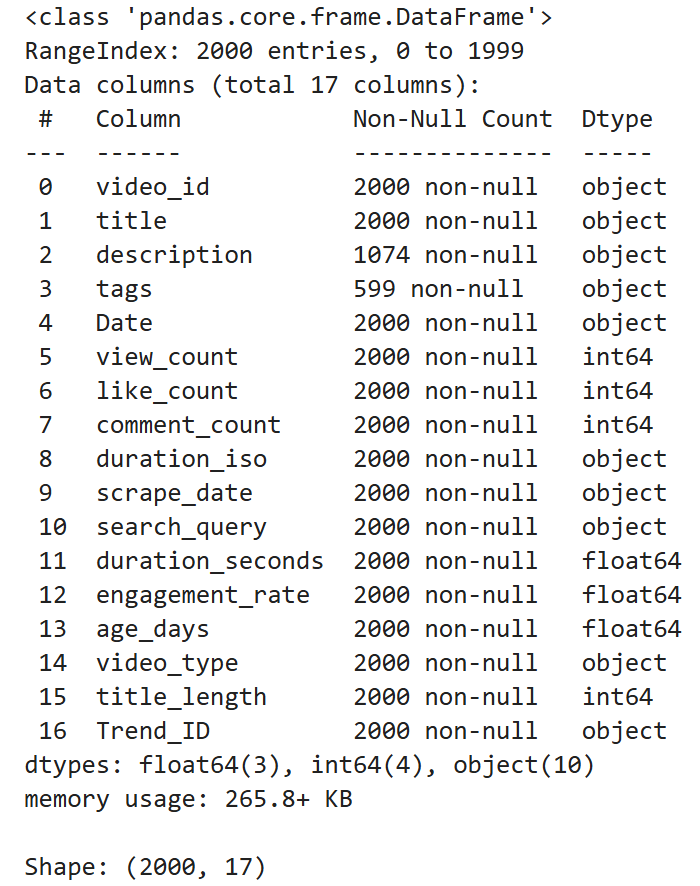
\includegraphics[width=\linewidth]{EDA_Figures/YoutubeDataSummary.png}
        \caption{YouTube Dataset Summary}
        \label{fig:youtube-summary}
    \end{subfigure}
    % Reddit in the center
    \begin{subfigure}[t]{0.32\textwidth}
        \centering
        \includegraphics[width=\linewidth]{EDA_Figures/RedditDataSummary.png}
        \caption{Reddit Dataset Summary}
        \label{fig:reddit-summary}
    \end{subfigure}
    % Google Trends on the right
    \begin{subfigure}[t]{0.32\textwidth}
        \centering
        \includegraphics[width=\linewidth]{EDA_Figures/GoogleTrendsSummary.jpg}
        \caption{Google Trends Dataset Summary}
        \label{fig:pytrends-summary}
    \end{subfigure}
    \caption{Cleaned dataset summaries for YouTube, Reddit, and Google Trends}
    \label{fig:dataset-summaries}
\end{figure}

The Dataset summaries in Figure 1 provide an overview of the cleaned data sources used in this analysis. The Youtube dataset contains 2,000 video entries with 17 standardized variables, including engagement metrics (views, likes, comments) and derived measures such as engagement rate, video age, and duration. The Reddit dataset includes 22,363 posts across multiple food-related subreddits, containing text features such as post titles, comment counts, and sentiment scores. And the Google Trends dataset provides weekly search interest values for each trend across several countries, allowing comparisons of temporal patterns in public attention. Together, these three datasets capture complementary aspects of online food trend activity: content creation and engagement (Youtube), discussion and sentiment (Reddit), and search interest (Google), forming the foundation for the exploratory analysis that follows. 

\begin{figure}[H]
    \centering
    
    % Top: YouTube
    \begin{subfigure}[t]{0.65\textwidth}
        \centering
        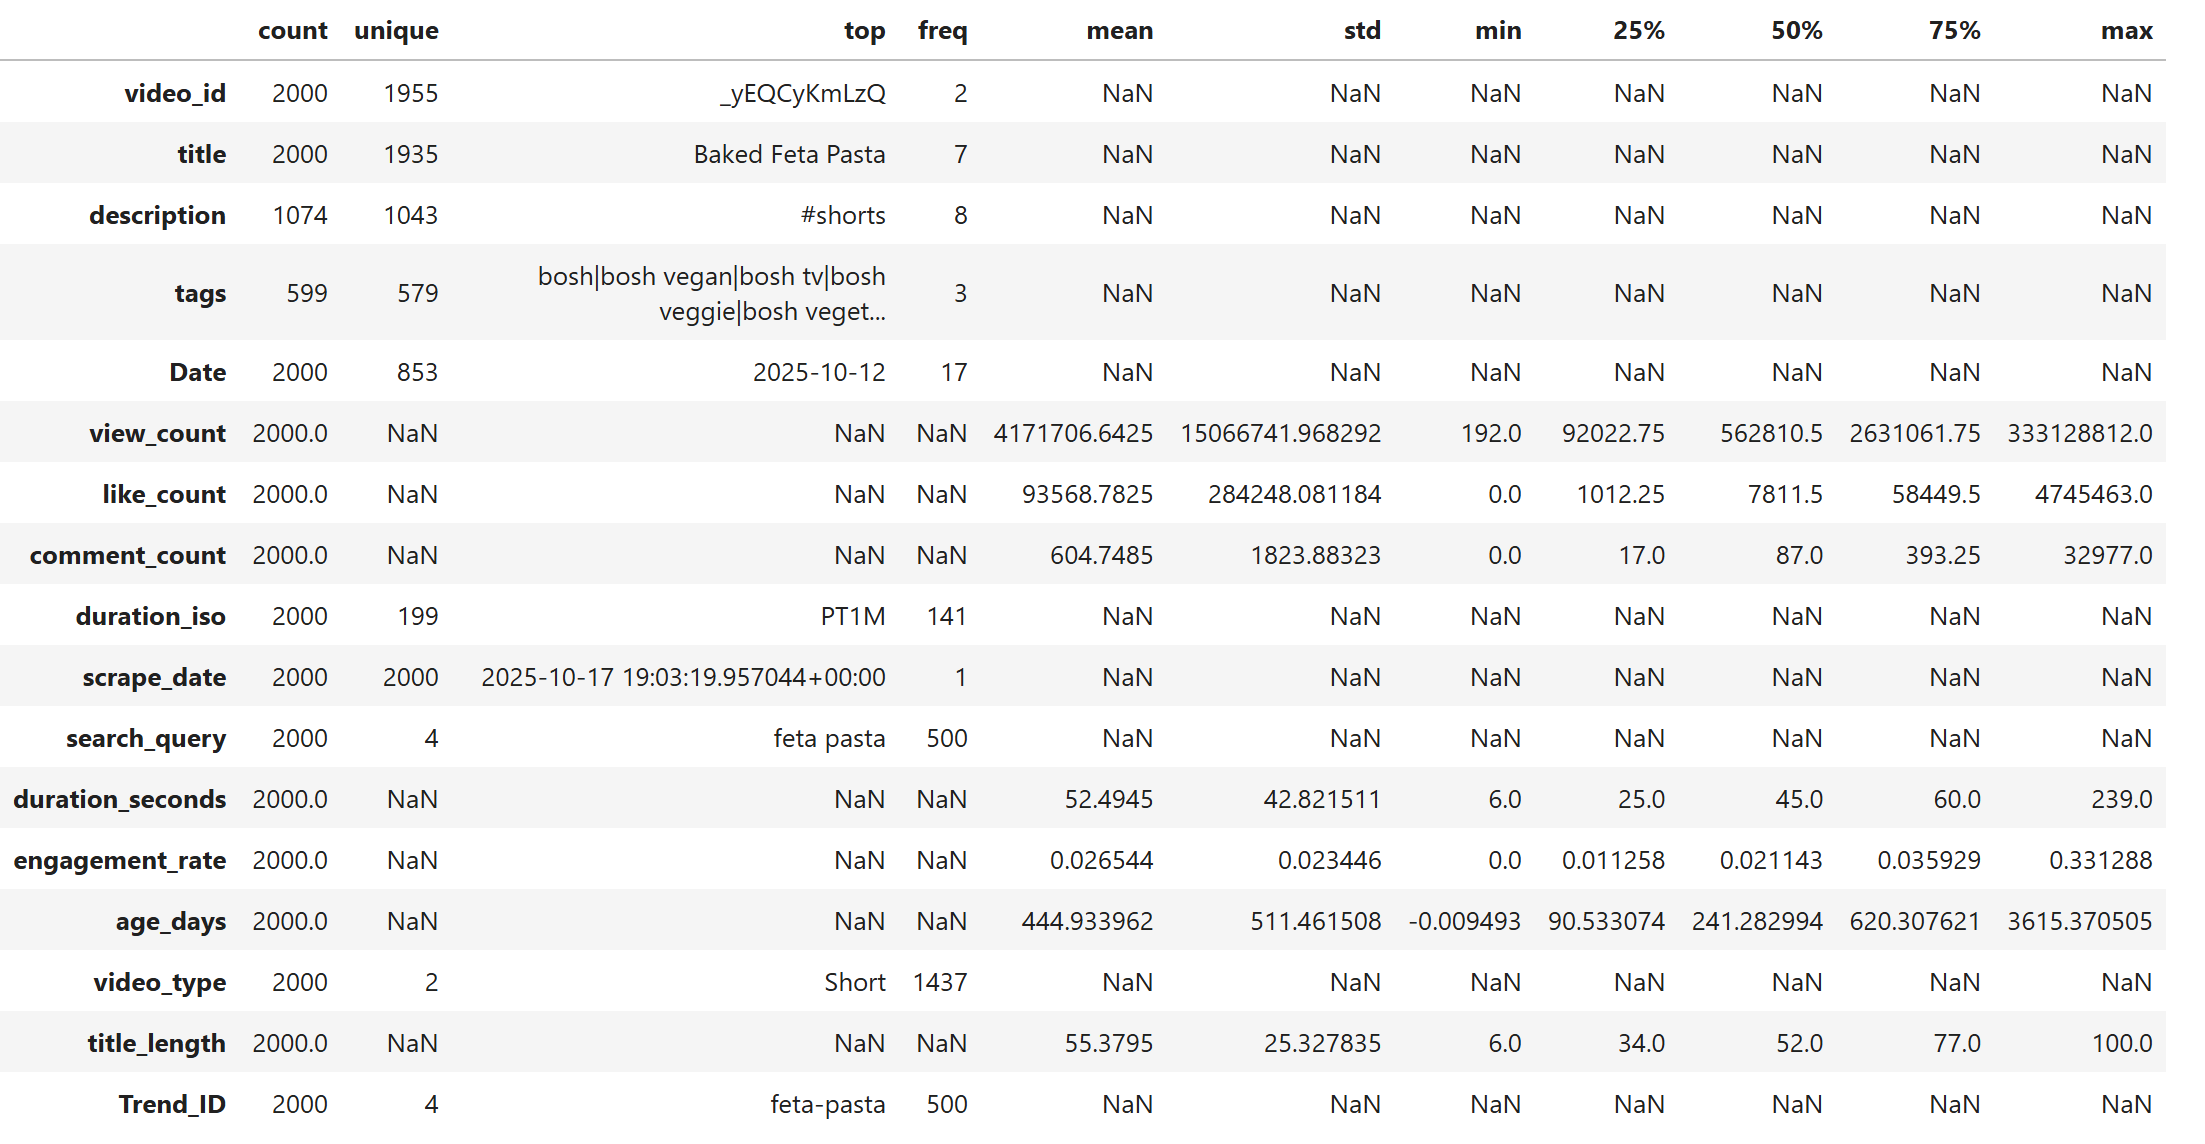
\includegraphics[width=\linewidth]{EDA_Figures/YoutubeDataStats.png}
        \caption{YouTube Dataset Summary}
        \label{fig:youtube-summary}
    \end{subfigure}

    \vspace{0.5cm} % Space between rows

    % Bottom: Reddit and Google Trends side by side
    \begin{subfigure}[t]{0.45\textwidth}
        \centering
        \includegraphics[width=\linewidth]{EDA_Figures/Reddit_Descriptive_Stats.png}
        \caption{Reddit Dataset Summary}
        \label{fig:reddit-summary}
    \end{subfigure}
    \hfill
    \begin{subfigure}[t]{0.45\textwidth}
        \centering
        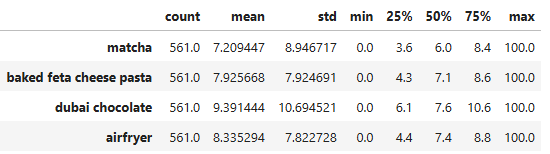
\includegraphics[width=\linewidth]{EDA_Figures/pytrends_stats.png}
        \caption{Google Trends Dataset Summary}
        \label{fig:pytrends-summary}
    \end{subfigure}

    \caption{Descriptive Statistics for YouTube, Reddit, and Google Trends}
    \label{fig:dataset-summaries}
\end{figure}

Figure 2 shows the descriptive statistics for the Youtube \citep{youtube_api}, Reddit \citep{reddit_api_praw}, and Google Trends datasets \citep{pytrends_api}. The Youtube data show wide variation in engagement metrics, with view counts averaging over four 4 million but ranging from hundreds to hundreds of millions, reflecting a highly skewed distribution typical of viral content. Reddit statistics indicate diverse posting activity and interaction levels across communities, while the Google Trends data show normalized search interest values between 0 and 100, representing relative popularity over time. Together, these summaries highlight the differing scales and behaviors captured across platforms, providing a quantitative foundation for the exploratory analyses that follow.

\newpage

\section{Exploratory Data Analysis}
\subsection{Trend Growth and Lifecycle Over Time}
To understand how food trends evolve over time, Youtube and Google Data were analyzed to observed when each trend emerged, peaked, and declined. These patterns reveal differences in how quickly trends gain visibility, how long they remain relevant, and whether they experience renewed interest over time.

\begin{figure}[H]
    \centering
    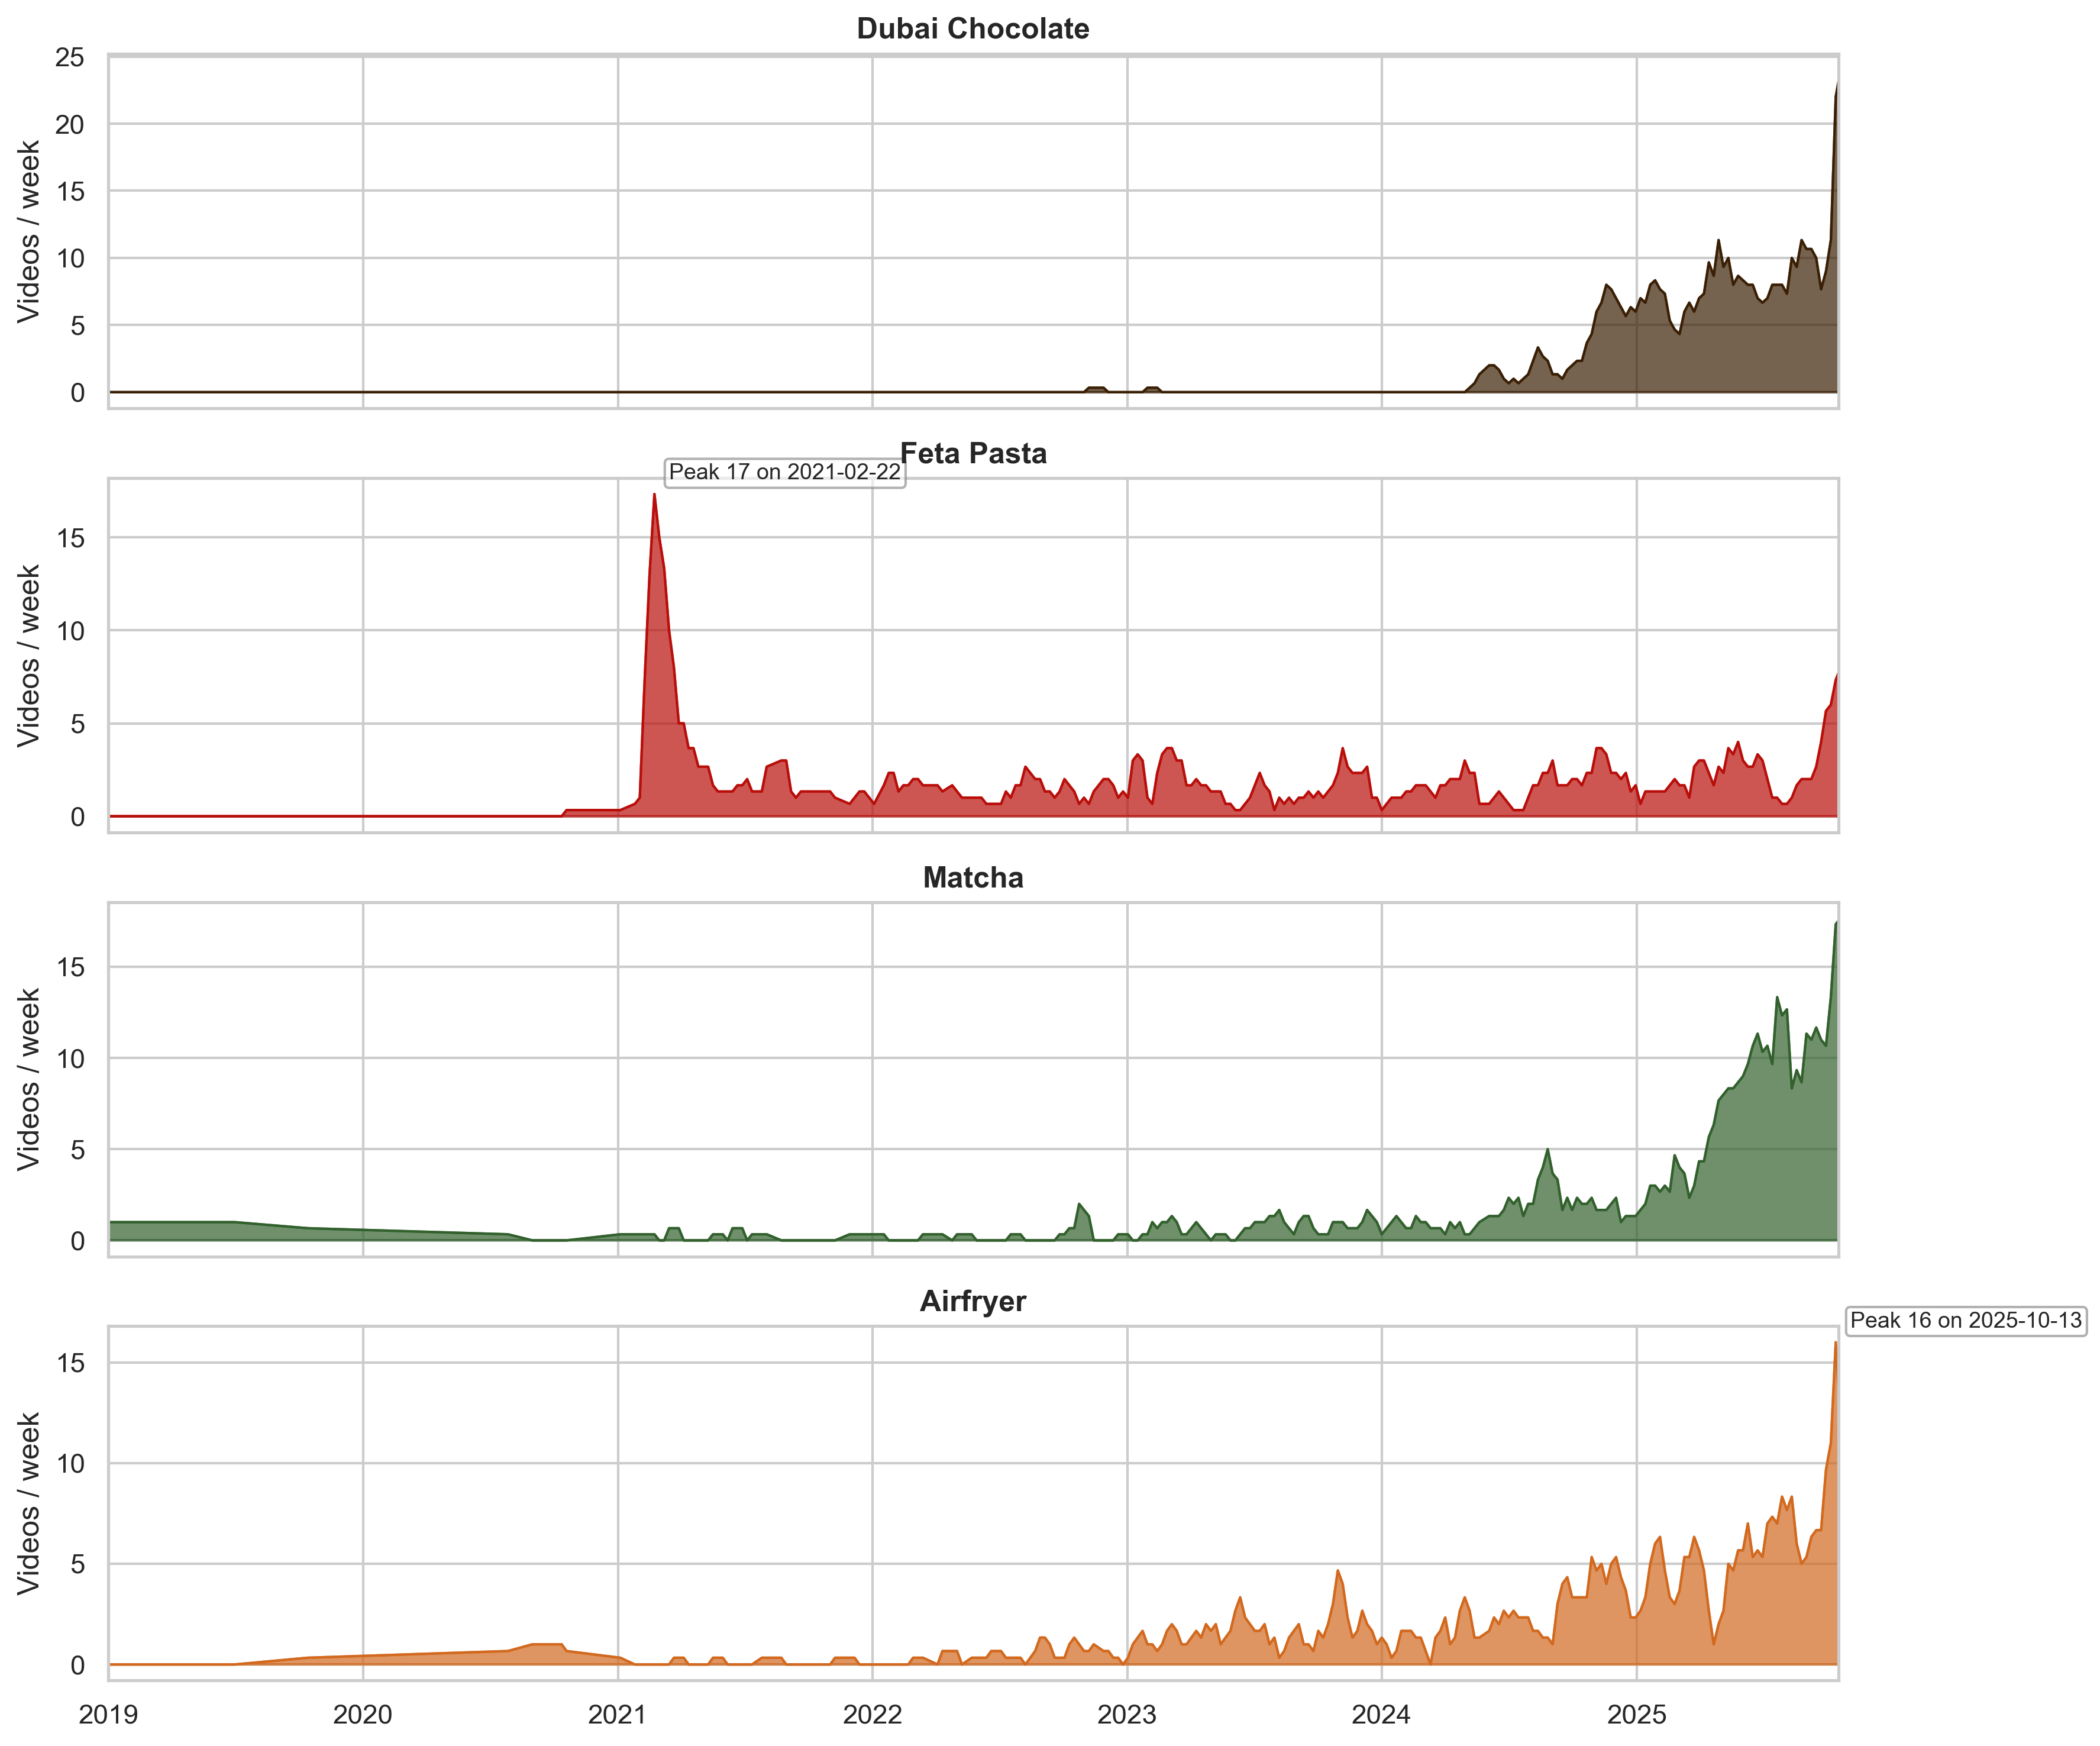
\includegraphics[width=\textwidth]{EDA_Figures/trend_plots.png}
    \caption{Weekly Youtube video trends for Dubai Chocolate, Feta Pasta, Matcha, and Airfryer.}
    \label{fig:trend_plots}
\end{figure}

Figure 3 shows the number of weekly Youtube videos uploaded for each trend between 2019 and 2025. The plot shows the distinct lifecycle patterns across the four food trends: feta pasta, matcha, Dubai Chocolate, and airfryer. The feta pasta trend experienced a dramatic and short-lived spike in early 2021, coinciding with its viral spread on social media during the COVID-19 lockdown period. This sudden burst of uploads reflects a rapid adoption and decline cycle typical of trends dirven by novelty and virality. In contrast, matcha and airfryer show steady growth beginning in 2022, with periodic fluctuations that indicate sustained audience interest over time. The Dubai chocolate trend, which appeared more recently, surged sharply in 2025 and quickly became the dominant topic in terms of weekly uploads. Overall, the total number of food-related uploads has increased sharply since 2023, reflecting Youtube's role as a platform for trend amplification and global sharing of food content. 

\begin{figure}[H]
    \centering
    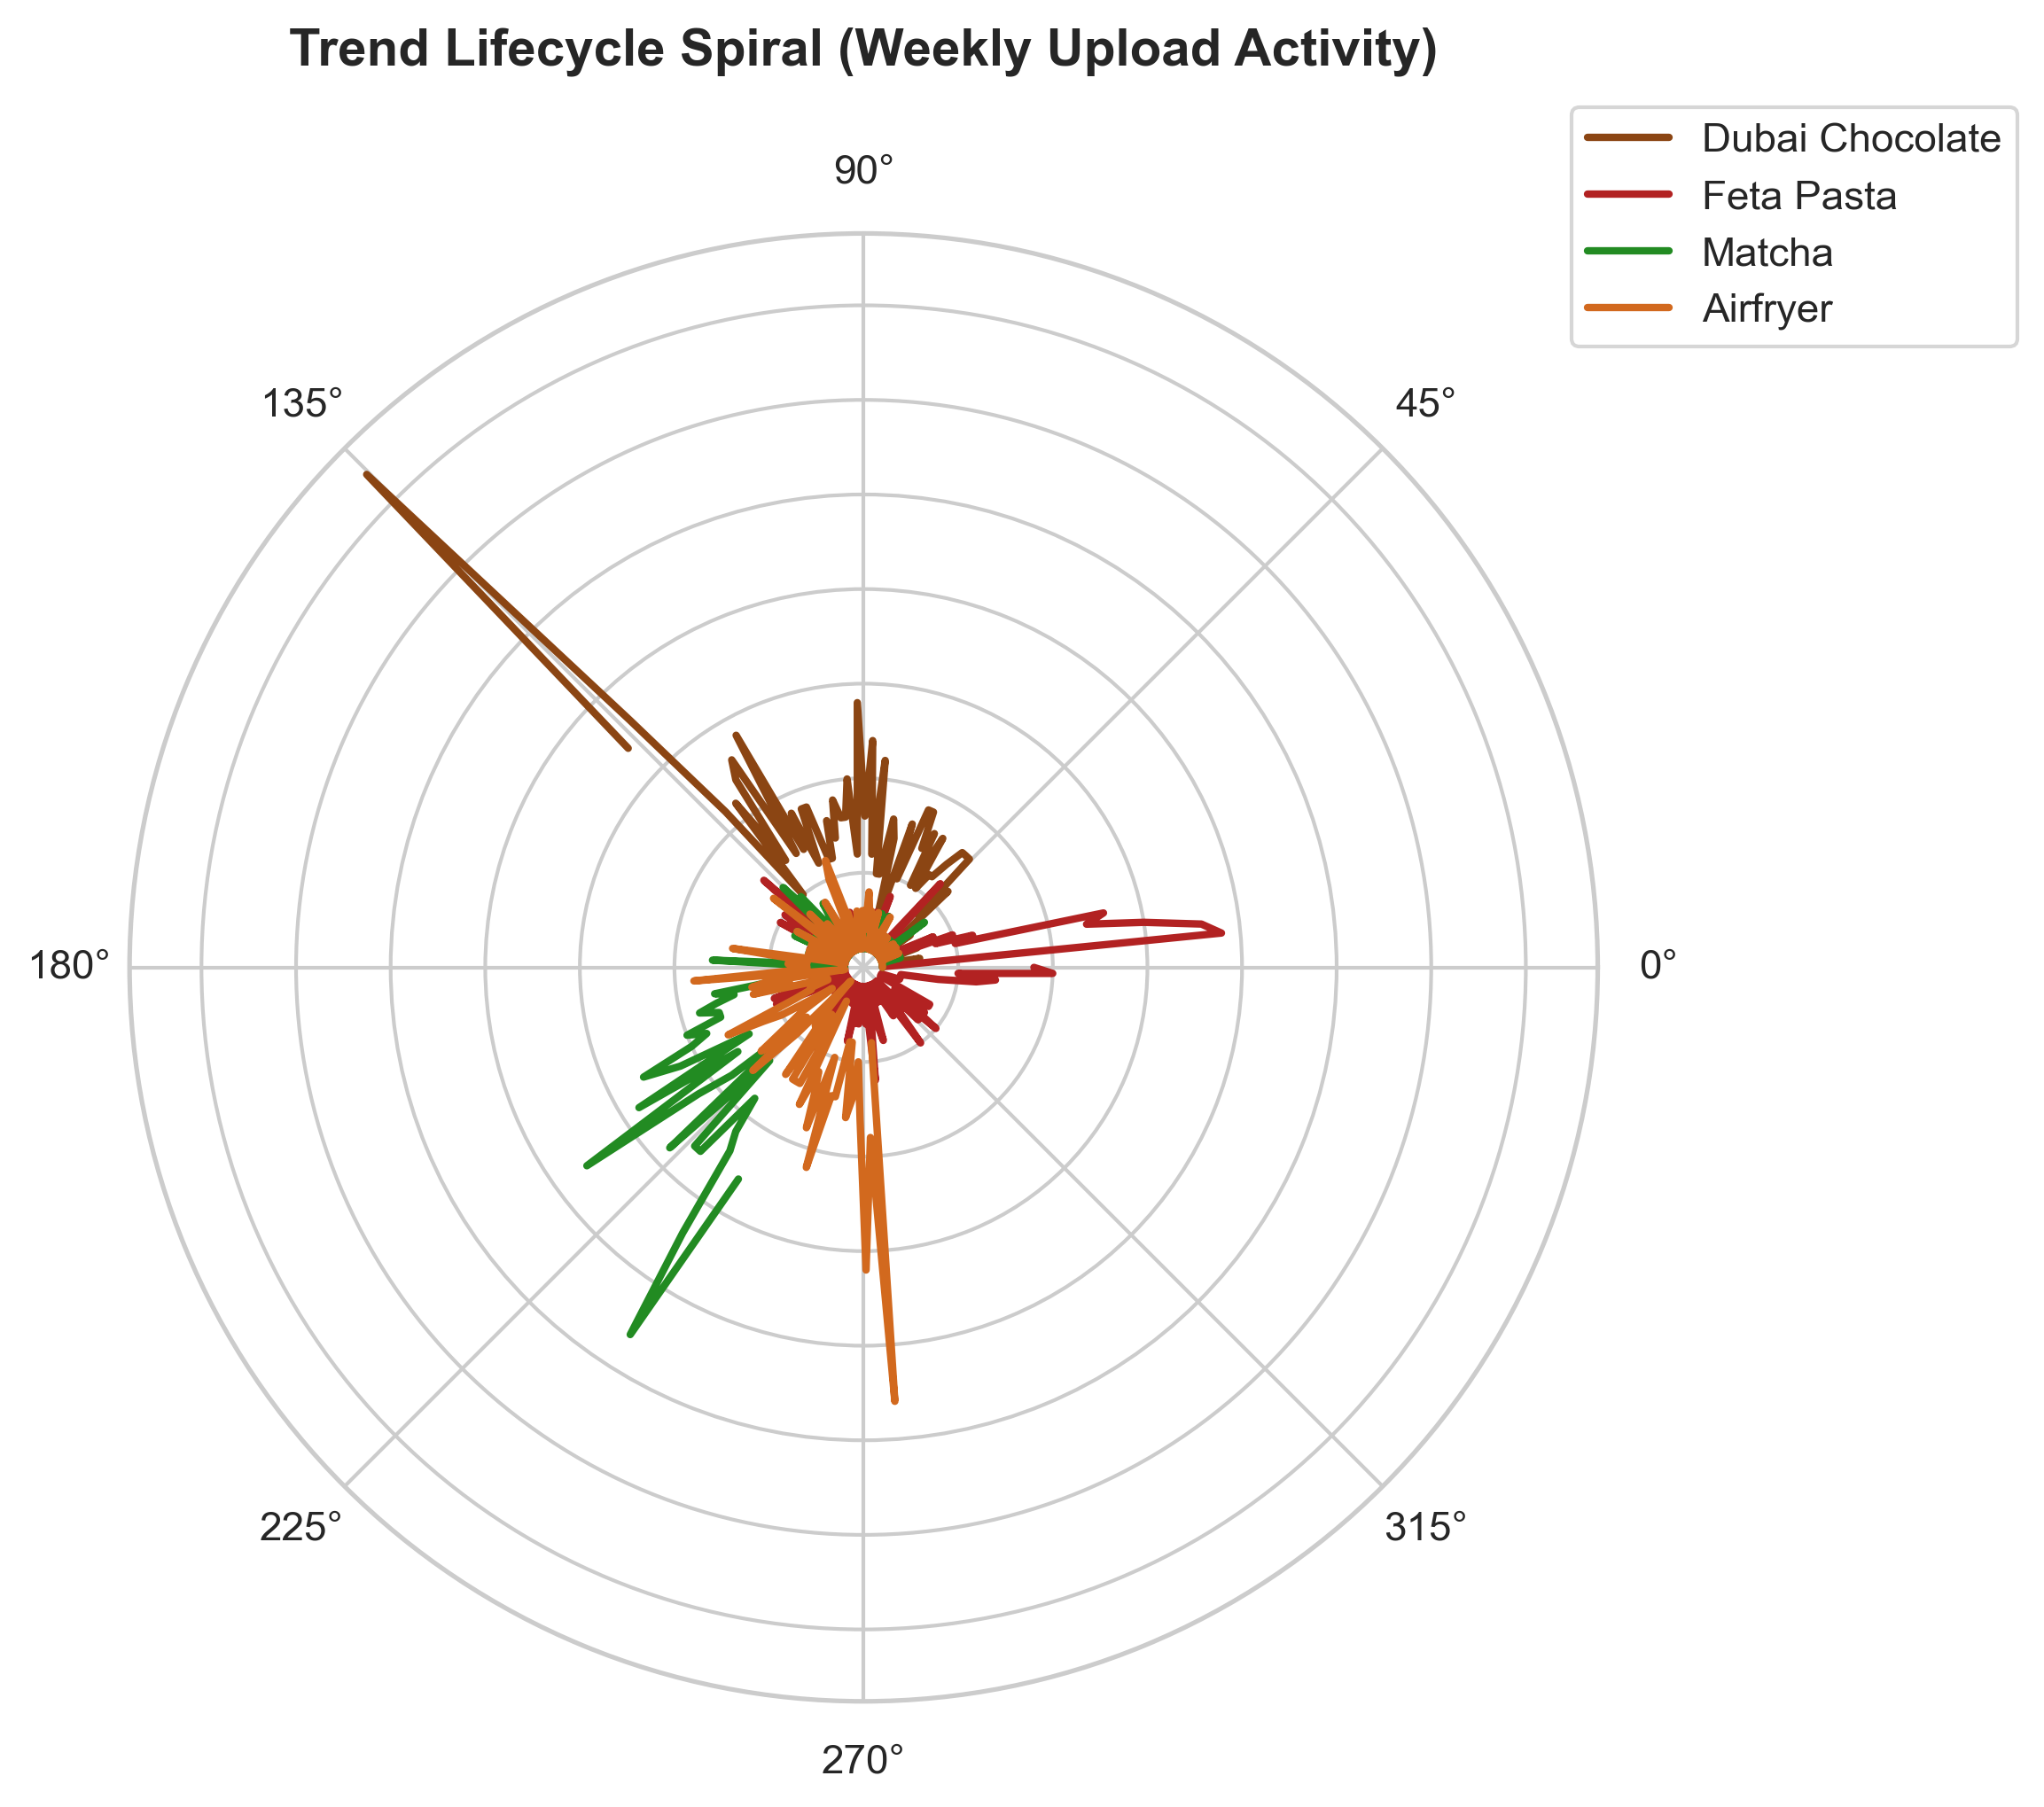
\includegraphics[width=\textwidth]{EDA_Figures/lifecycle_spiral.png}
    \caption{Lifecycle of Trends by Weekly Upload Activity}
    \label{fig:lifecycle_spiral}
\end{figure}

This visualization presents a spiral chart of weekly Youtube upload activity. Each line traces the progression of content creation over time, starting from a trend's emergence and expanding outward as weekly uploads accumulate. The spiral visualization provides a clear representation of the differing lifecycles among the four trends. Feta Pasta shows a brief but intense burst of uploads concentrated near its early peak, indicating a rapid viral cycle that faded quickly. Matcha and Airfryer form broader, more evenly distributed spirals, reflecting sustained growth and long-term relevance. Dubai Chocolate, meanwhile, expands sharply in the outer layers, suggesting a more recent but rapidly accelerating phase of activity.

\begin{figure}[H]
    \centering
    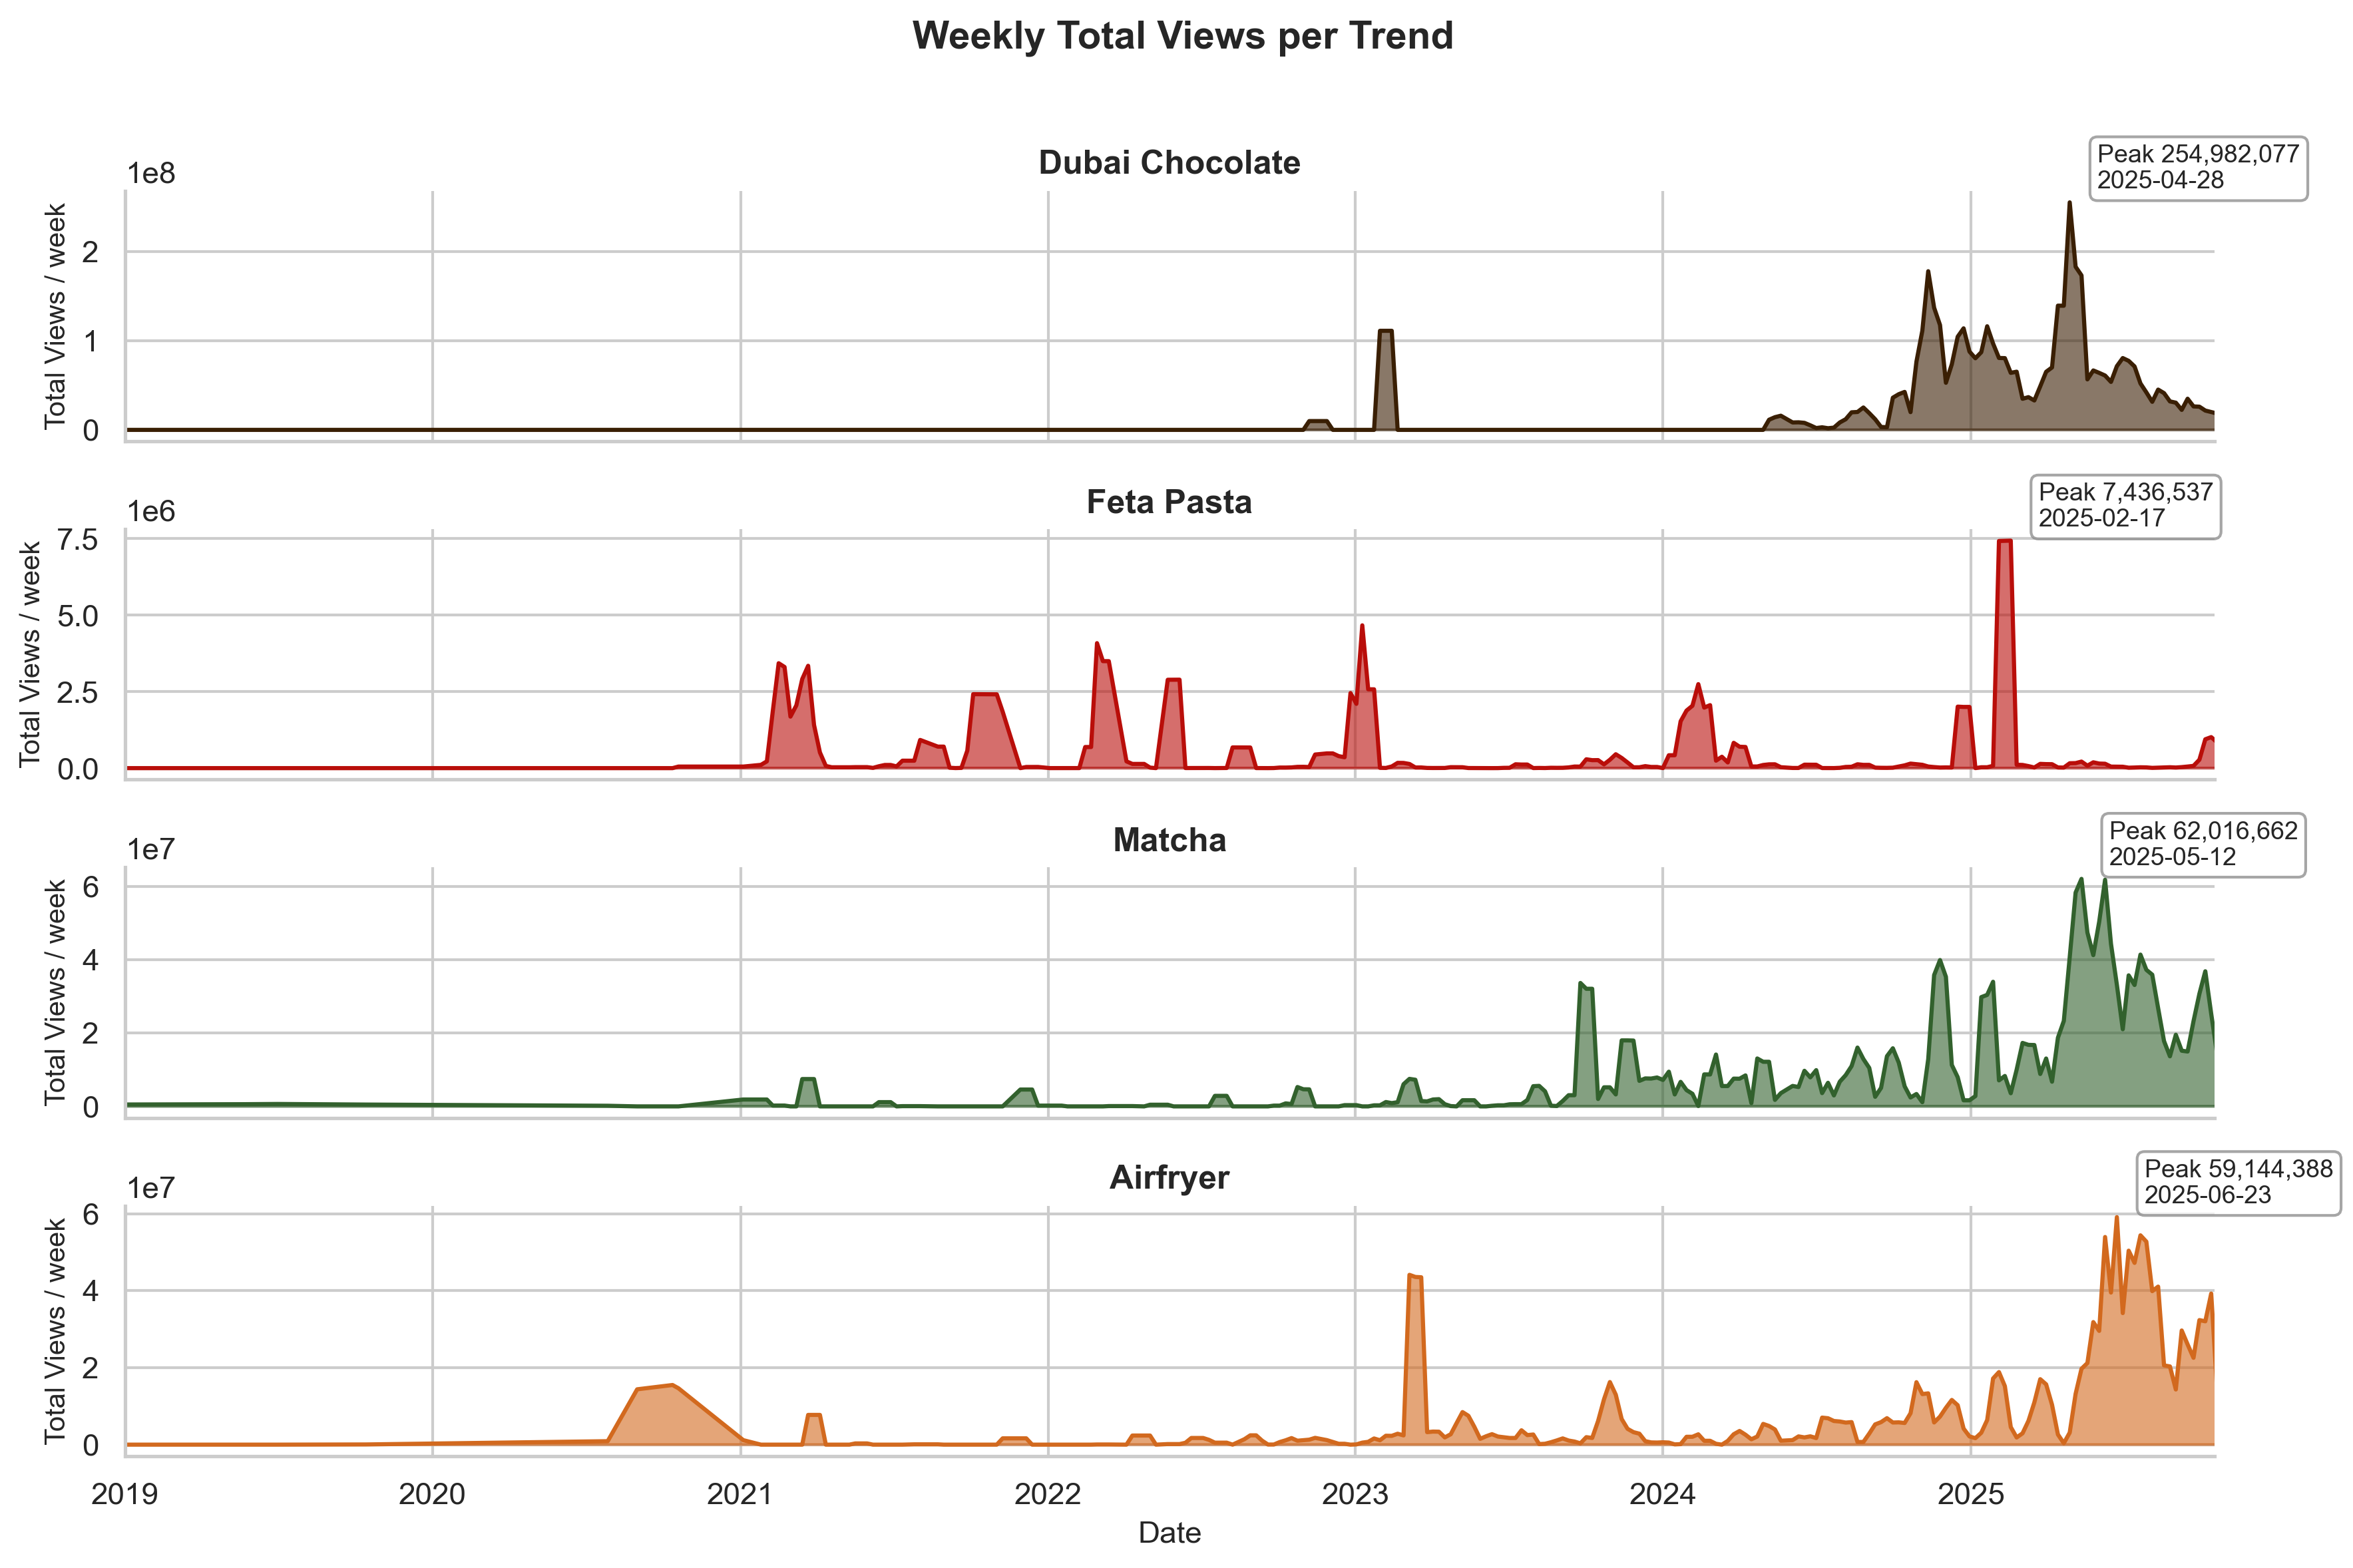
\includegraphics[width=\textwidth]{EDA_Figures/trend_plots2.png}
    \caption{Weekly Youtube views for Dubai Chocolate, Feta Pasta, Matcha, and Airfryer.}
    \label{fig:trend_plots2}
\end{figure}

Figure 5 shows weekly total views per trend, illustrating how audience attention aligns with content production. Dubai chocolate achieved the highest single-week peak of approximately 255 million views in April 2025, surpassing the other trends. Matcha also saw significant spikes in 2024 and 2025, suggesting cycles of renewed interest possibly tied to cultural or seasonal factors. Feta pasta peaked and declined multiple times between 2021 and early 2025, where it reached the highest peak of 7.5 million views in February 2025, eventually fading away. Airfryer maintained a moderate but consistent level of attention, showing that some trends achieve longevity through sustained utility. The combined patterns from both figures show that food trends often follow distinct lifecycles: some rise quickly and decline after saturation, while others maintain relevance for a longer period of time. 


\begin{figure}[H]
    \centering
    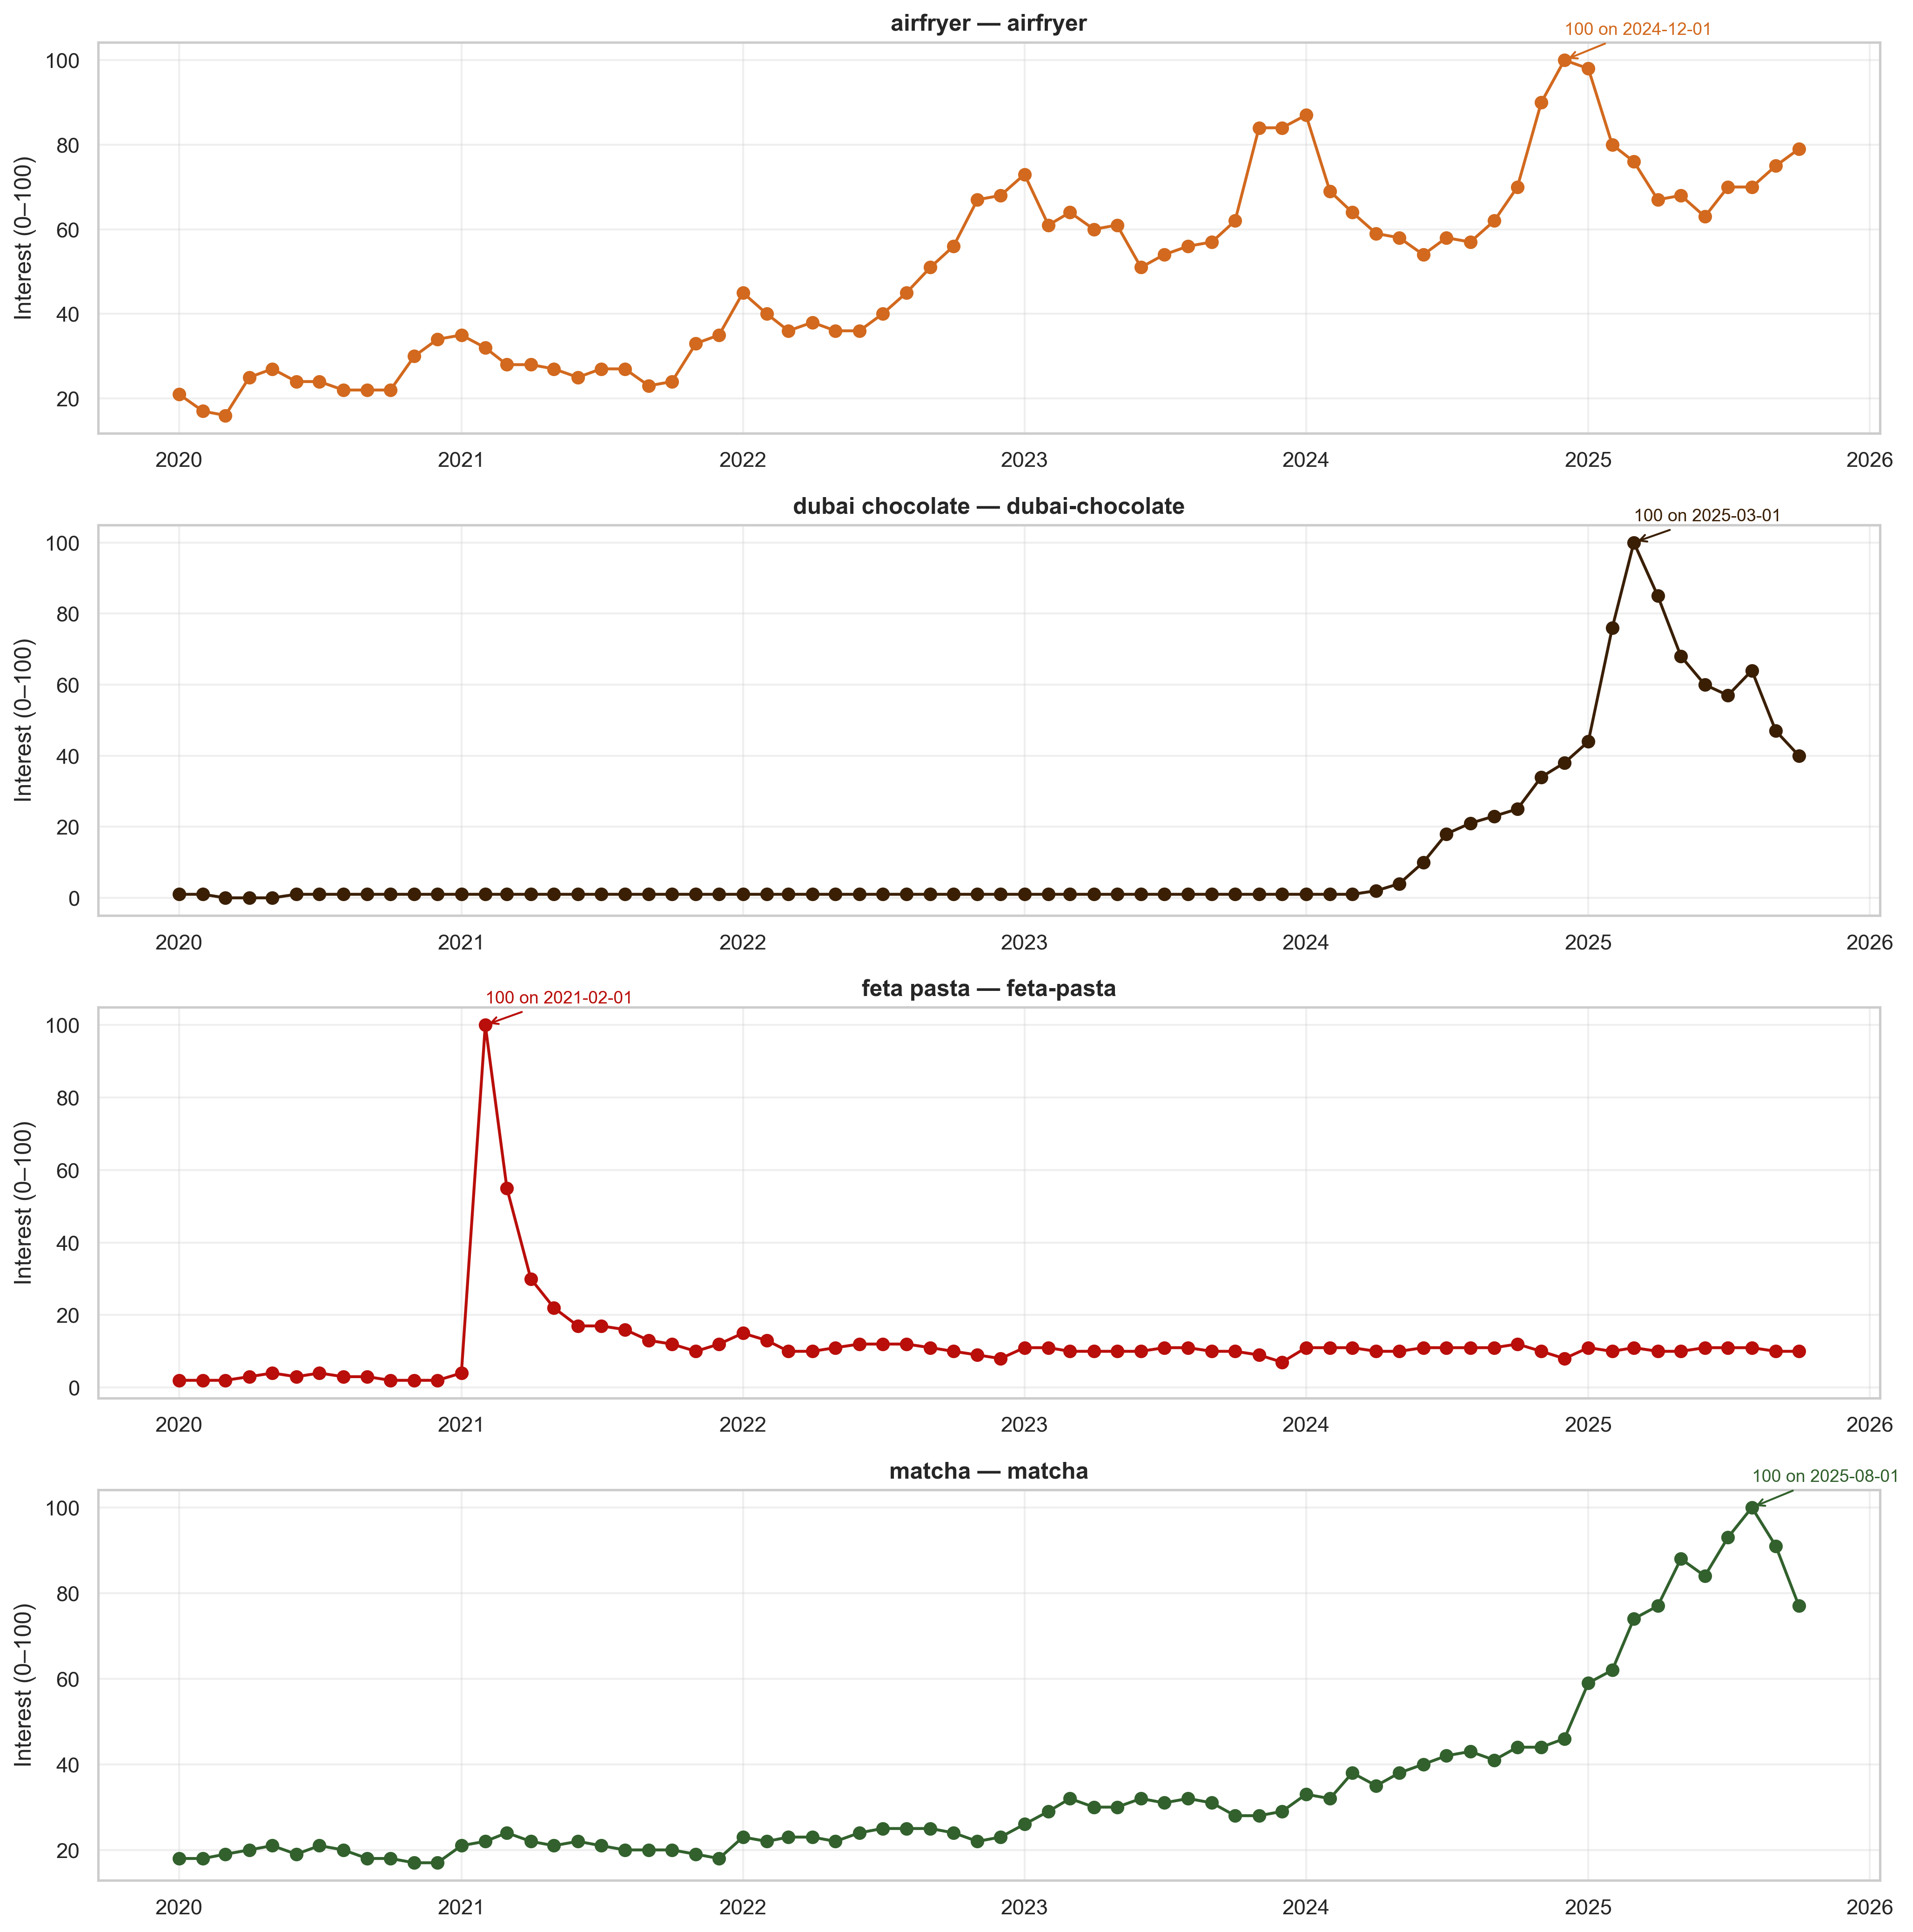
\includegraphics[width=\textwidth]{EDA_Figures/pytrends_searchInterest.png}
    \caption{Search Interest Over Time for Matcha, Dubai Chocolate and Baked Feta Cheese Pasta}
    \label{fig:pytrends_SI}
\end{figure}

Figure 6 depicts global search interest for the four food trends over a weekly time span from 2020 to 2025 and highlights their unique lifecycle appearances. Air Fryer has had its fair share of ups and downs and has been consistent in its repeated growth activity and peak interest since early 2022, which suggests that there is sustained interest in Air Fryers globally and consumers accepted and adapted to using this appliance, rather than just became interested socially to replace previous food preparation. Dubai Chocolate had sudden growth interest in early 2025, after a few years of very low interest activity, highlighting how certain trends can emerge and reappear due to renewed viral behavior. Baked Feta Cheese Pasta had a rapid and short burst in global growth interest, due to "going viral" primarily through social media during COVID-19 lockdowns, and generally returned to pre-pandemic interest levels within just a few months. Matcha appears to have more steady, longer-term growth interest, with smaller bursts of interest in 2024, demonstrating the semi-annual rise and fall of healthy, culturally engaging practices. 

Overall, comparing across the three time series reveals different trend archetypes: Feta Pasta as a short-term viral phenomena, Matcha as a slowly maturing global movement, and Dubai Chocolate as a recurring niche trend, augmented by social media virality.

\subsection{Audience Reach and Engagement Patterns}
While temporal trends show when food content becomes popular, audience engagement metric reveal how users interact with that content once it appears. Youtube's engagement data, which includes views, likes, comments, and calculated engagement rates highlight the uneven attention distribution typical of trending media and help distinguish between broad visibility and active viewer participation. 

\begin{figure}[H]
    \centering
    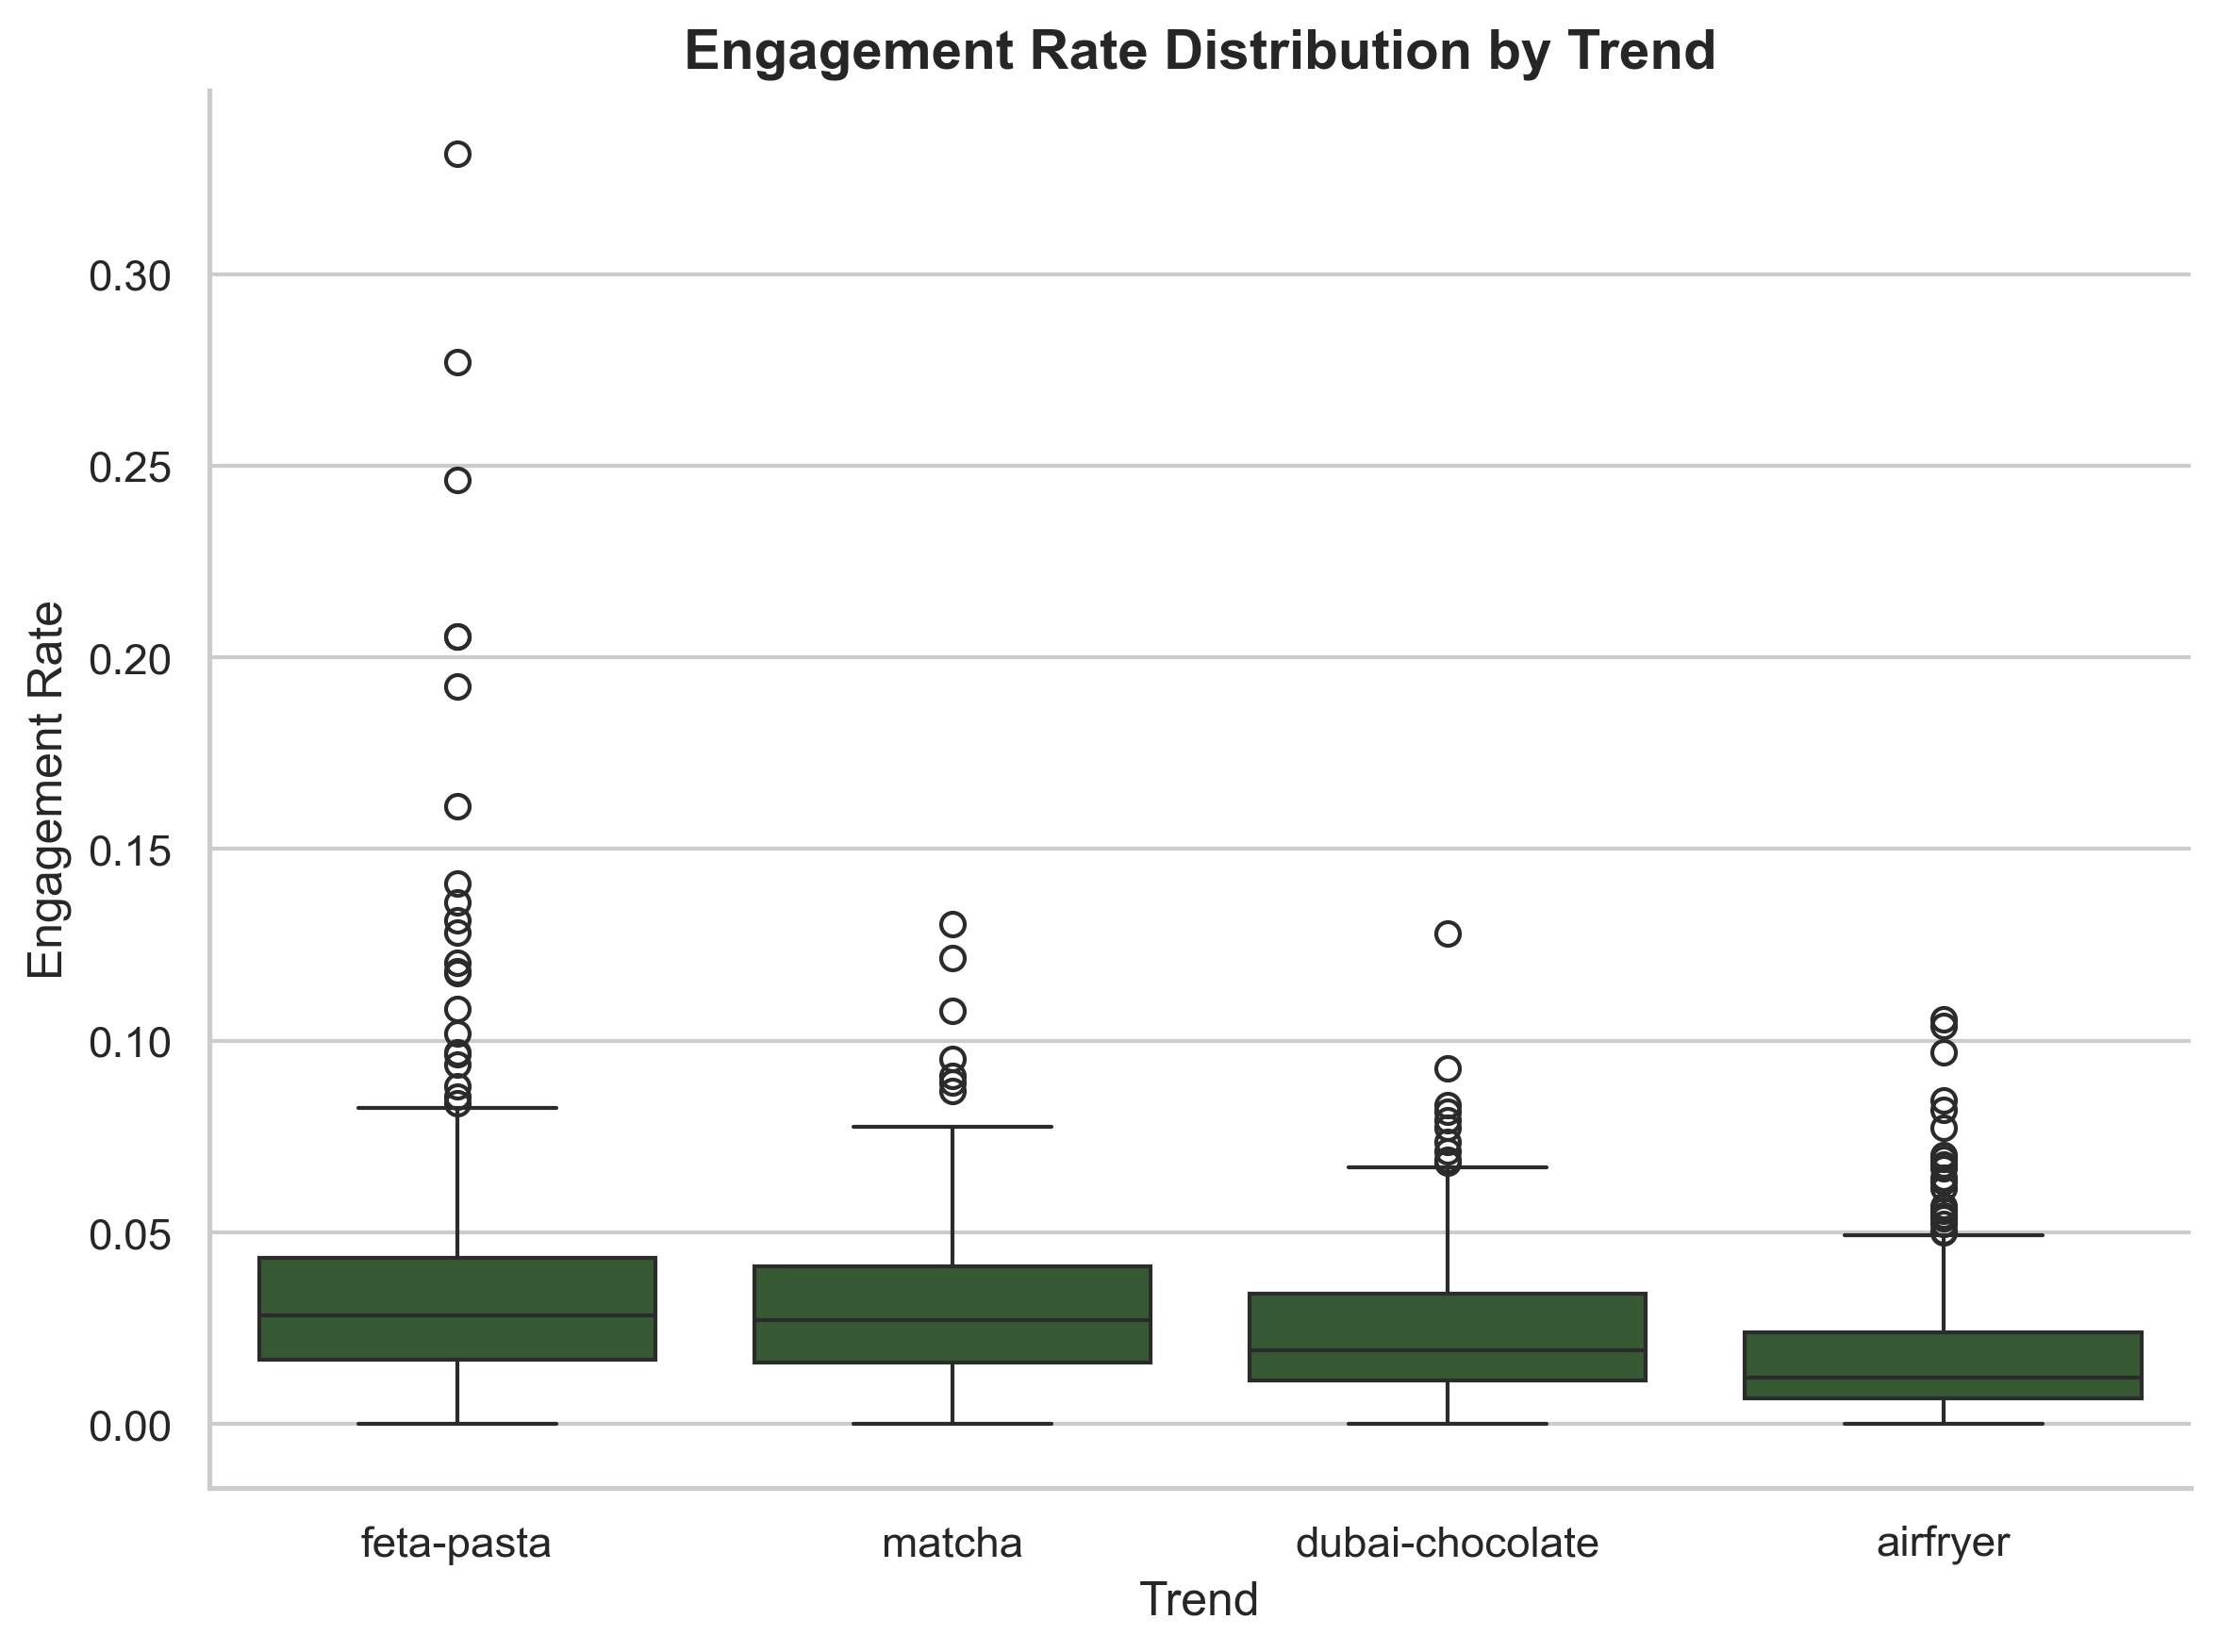
\includegraphics[width=\textwidth]{EDA_Figures/engagement_rate.png}
    \caption{Engagement Rate Distribution}
    \label{fig:engagement_rate}
\end{figure}

Figure 7 shows the distribution of engagement rates across all 4 trends. Each bos represents the central range of engagement rates, while outliers capture videos that achieved unusually high interaction relative to their total views. From this visualization, it is clear that the majority of videos have engagement rates clustered below 0.05 (5\%), indicating that only a small fraction of viewers typically interact through likes or comments. However, each trend exhibits a few extreme outliers exceeding 0.10, representing highly viral videos that sparked audience response. Among the four, Feta pasta and Matcha showed higher variability, suggesting that these trends generated a wider range of viewer engagement, likely due to their novelty and timing during peak online virality periods. These results emphasize the skewed nature of online engagement: most videos receive modest likes and comments, while a handful show better user interactions.

\begin{figure}[H]
    \centering
    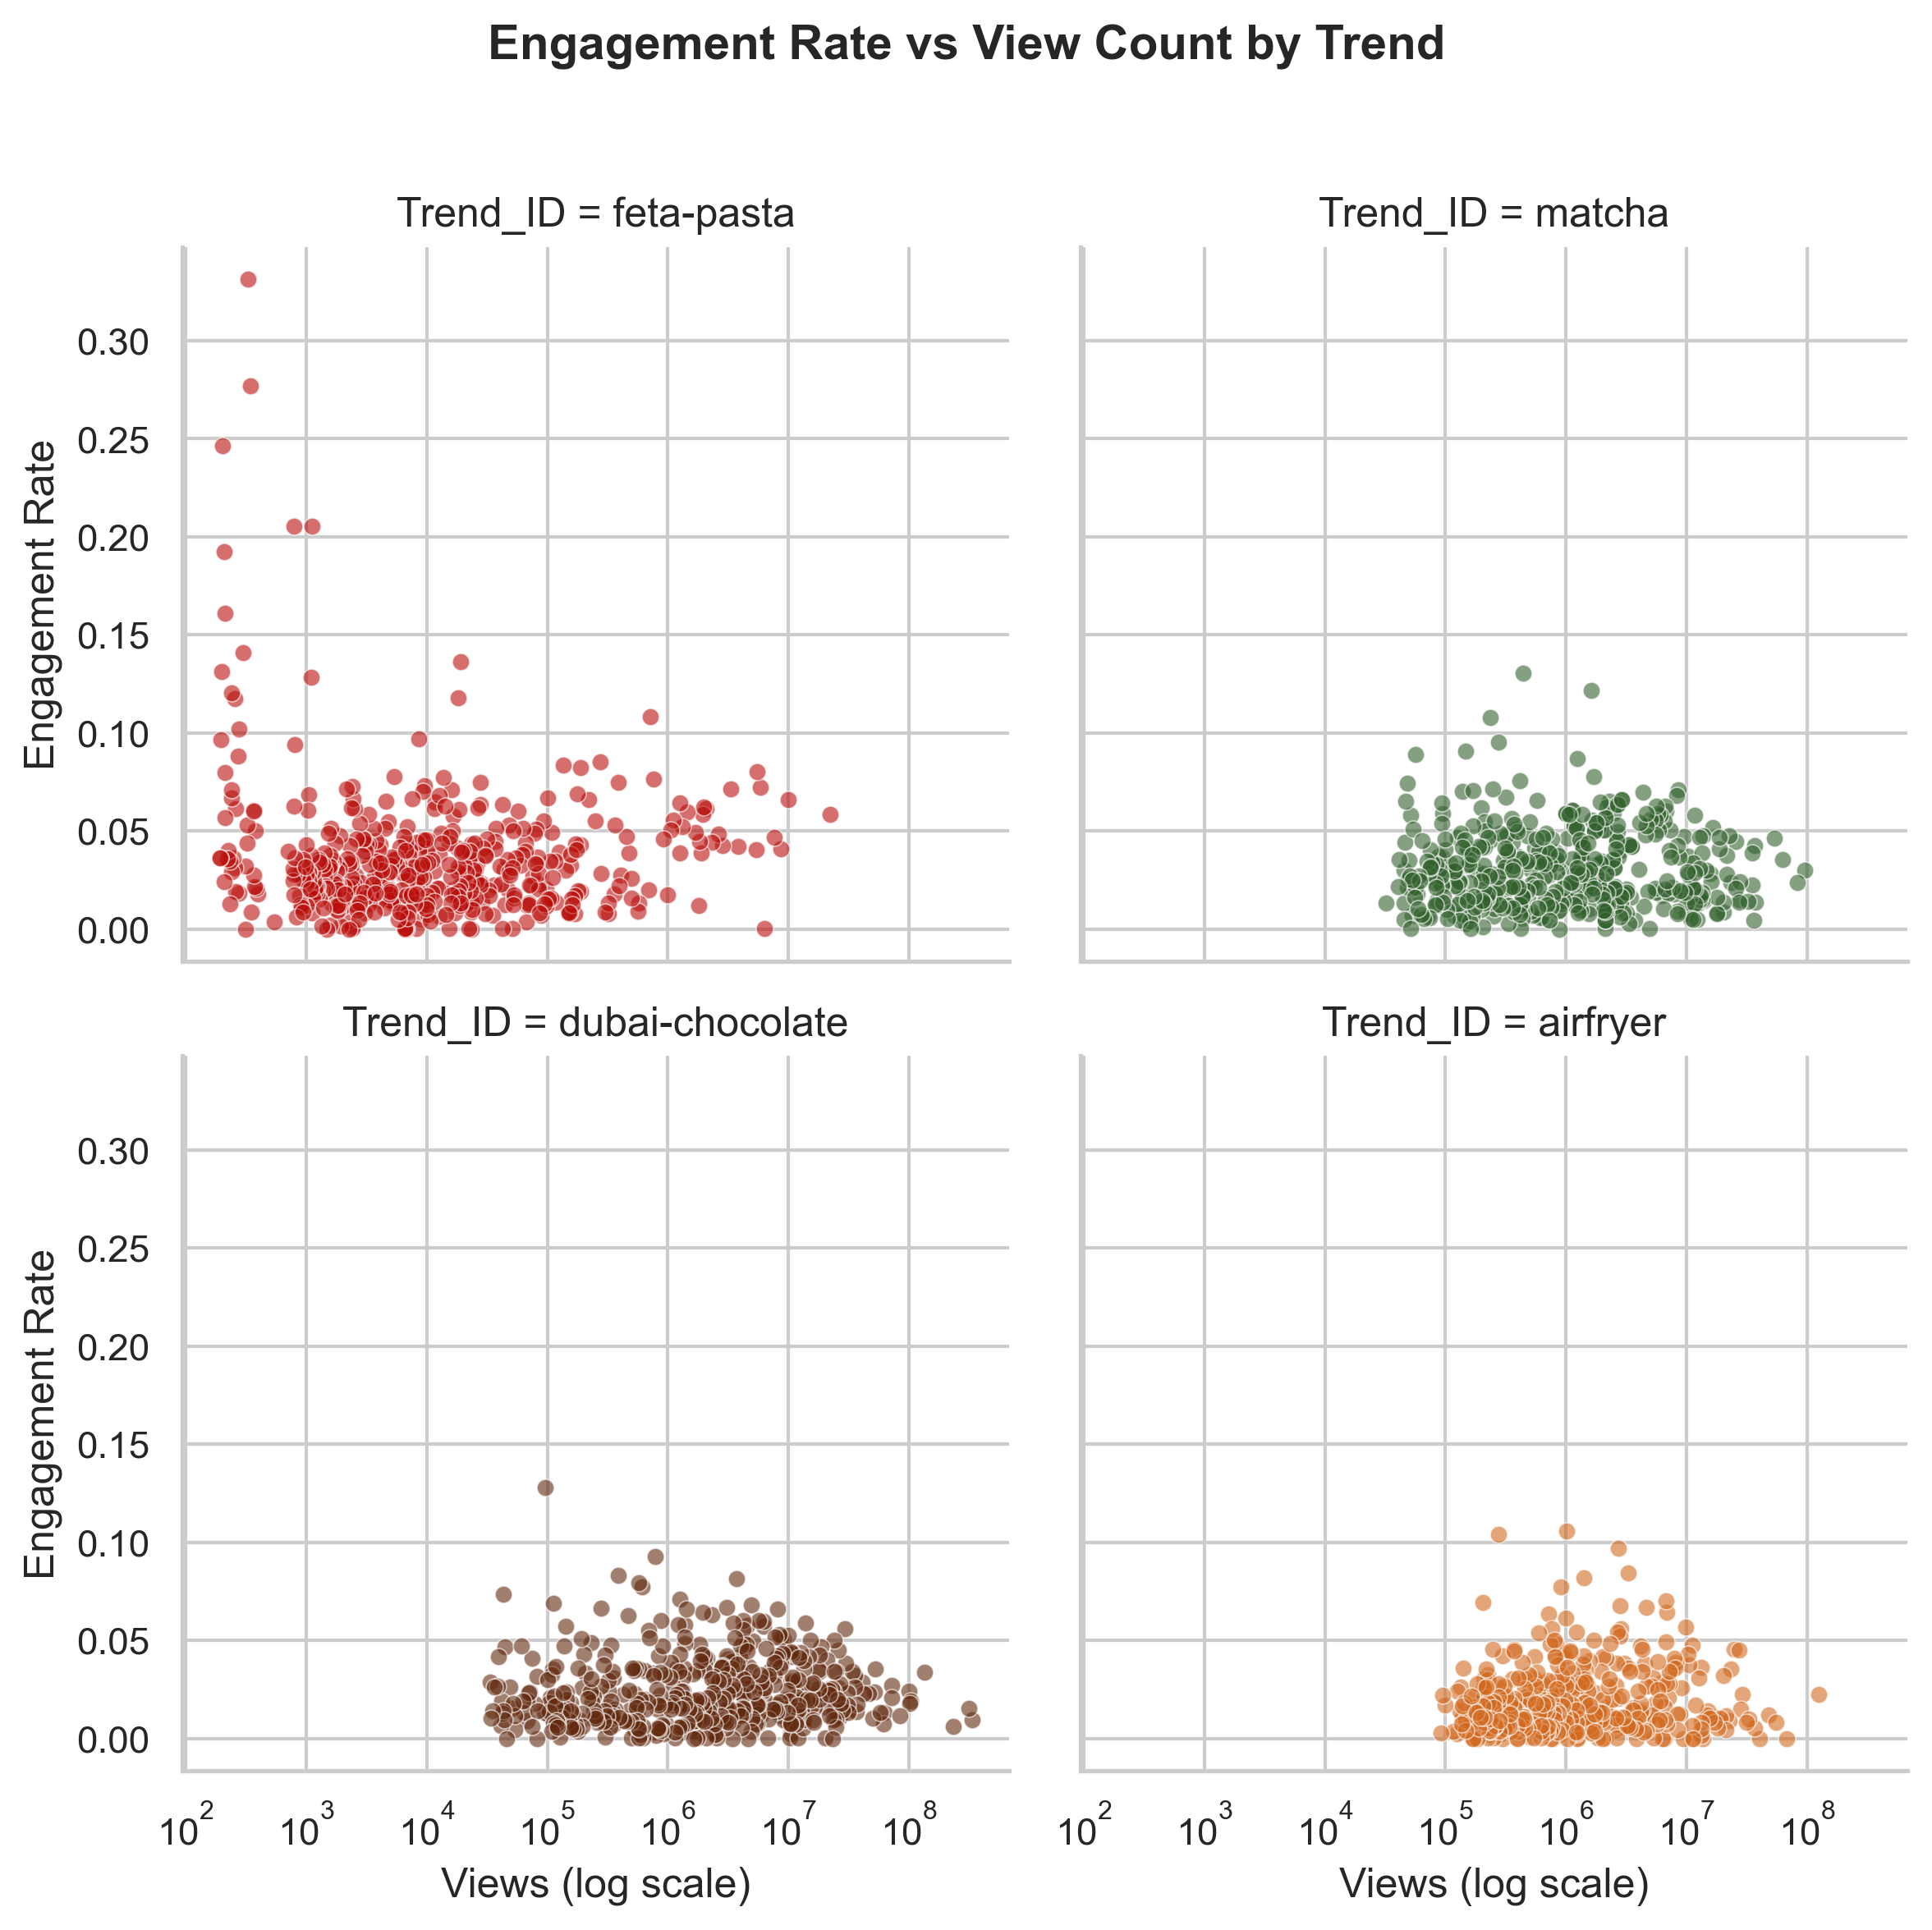
\includegraphics[width=\textwidth]{EDA_Figures/engagement_views.png}
    \caption{Comparing Engagement Rate to Total View Count}
    \label{fig:engagement_views}
\end{figure}

Each scatterplot in figure 8 shows how interaction levels vary as videos attract larger audiences. Across all four trends, engagement rate remains relatively stable across different view counts, suggesting that the level of interaction does not strongly depend on how widely a video is viewed. Most videos, regardless of hundreds, thousands, or millions of views, maintain engagement rates within a narrow range between 0.01 and 0.10. This horizontal spread indicates that audience interaction scales proportionally with viewership rather than diminishing as videos go viral. 

Feta pasta shows a wider spread of engagement at moderate view counts, suggesting occasional spikes in viewer response during their viral phases. In contrast, other trends show tighter groupings at mid-high range views, reflecting steadier audience behavior over time. The logarithmic view scale also emphasizes how a small number of highly viral videos dominate total reach. Overall, the figure shows that creators can achieve strong engagement even without extremely high view counts. 

\begin{figure}[H]
    \centering
    \includegraphics[width=\textwidth]{EDA_Figures/PytrendsOverTime.pdf}
    \caption{Weekly Google searches for Matcha, Dubai Chocolate, and Airfryer}
    \label{fig:engagement_views}
\end{figure}

Figure 9 illustrates the worldwide and country-specific Google search trends for Matcha, Dubai Chocolate, and Air Fryer between 2015 and 2025. 
The trend for Matcha began its steep and steady rise around 2018, but there has been an observable spike in worldwide interest since 2023. The upward pattern clearly indicates the shift of Matcha from niche wellness ingredient into a global phenomenon (nationwide or global) that changed health trends. The jump in worldwide interest following 2023 shows a revived interest through social media health movements and café trends, particularly in the UK, USA, and South Korea. In these countries, matcha-based beverages became extremely trendy. 

On the other hand, the trend for Dubai Chocolate had a very different late, but exponential spike in 2025. Searches from around the world were fairly flat throughout this observed period, but in early 2025 there was an enormous spike exemplifying how quickly this topic regained viral attention, largely driven by online exposure and sharing from popular influencers. The spike was visible around the world and especially in the UAE, showing that the local and then worldwide attention gained traction quickly.

The trend for Air Fryer continues to demonstrate sustained cyclical growth starting around 2019, with Air Fryer reaching a first peak during the pandemic period while cooking at home interest exploded in 2021. The interest in the Air Fryer continued to grow in 2022-2024 and suggests that Air Fryer has changed from a novelty item to a normal household kitchen appliance. While global and US interest remains strong during this time, seasonal and holiday fluctuations fall within the time periods of the cooking and healthy cooking trends.

Overall, the three figures highlight different trends in diffusion, whereby Matcha is reflected as a globally and steadily trending health benefit, Dubai Chocolate is a sudden breakthrough experience, and Air Fryer is seen as an innovative product that is practical and will ultimately have long-term relevance to consumers.


\subsection{Content Characteristics and Performance}
Beyond overall engagement, it is important to understand how specific content features influence visibility and audience response. Taking a look at factors such as video type, duration, age, and title length and how they shape viewer interaction across the four food trends.

\begin{figure}[H]
    \centering
    % First image
    \begin{minipage}[t]{0.48\textwidth}
        \centering
        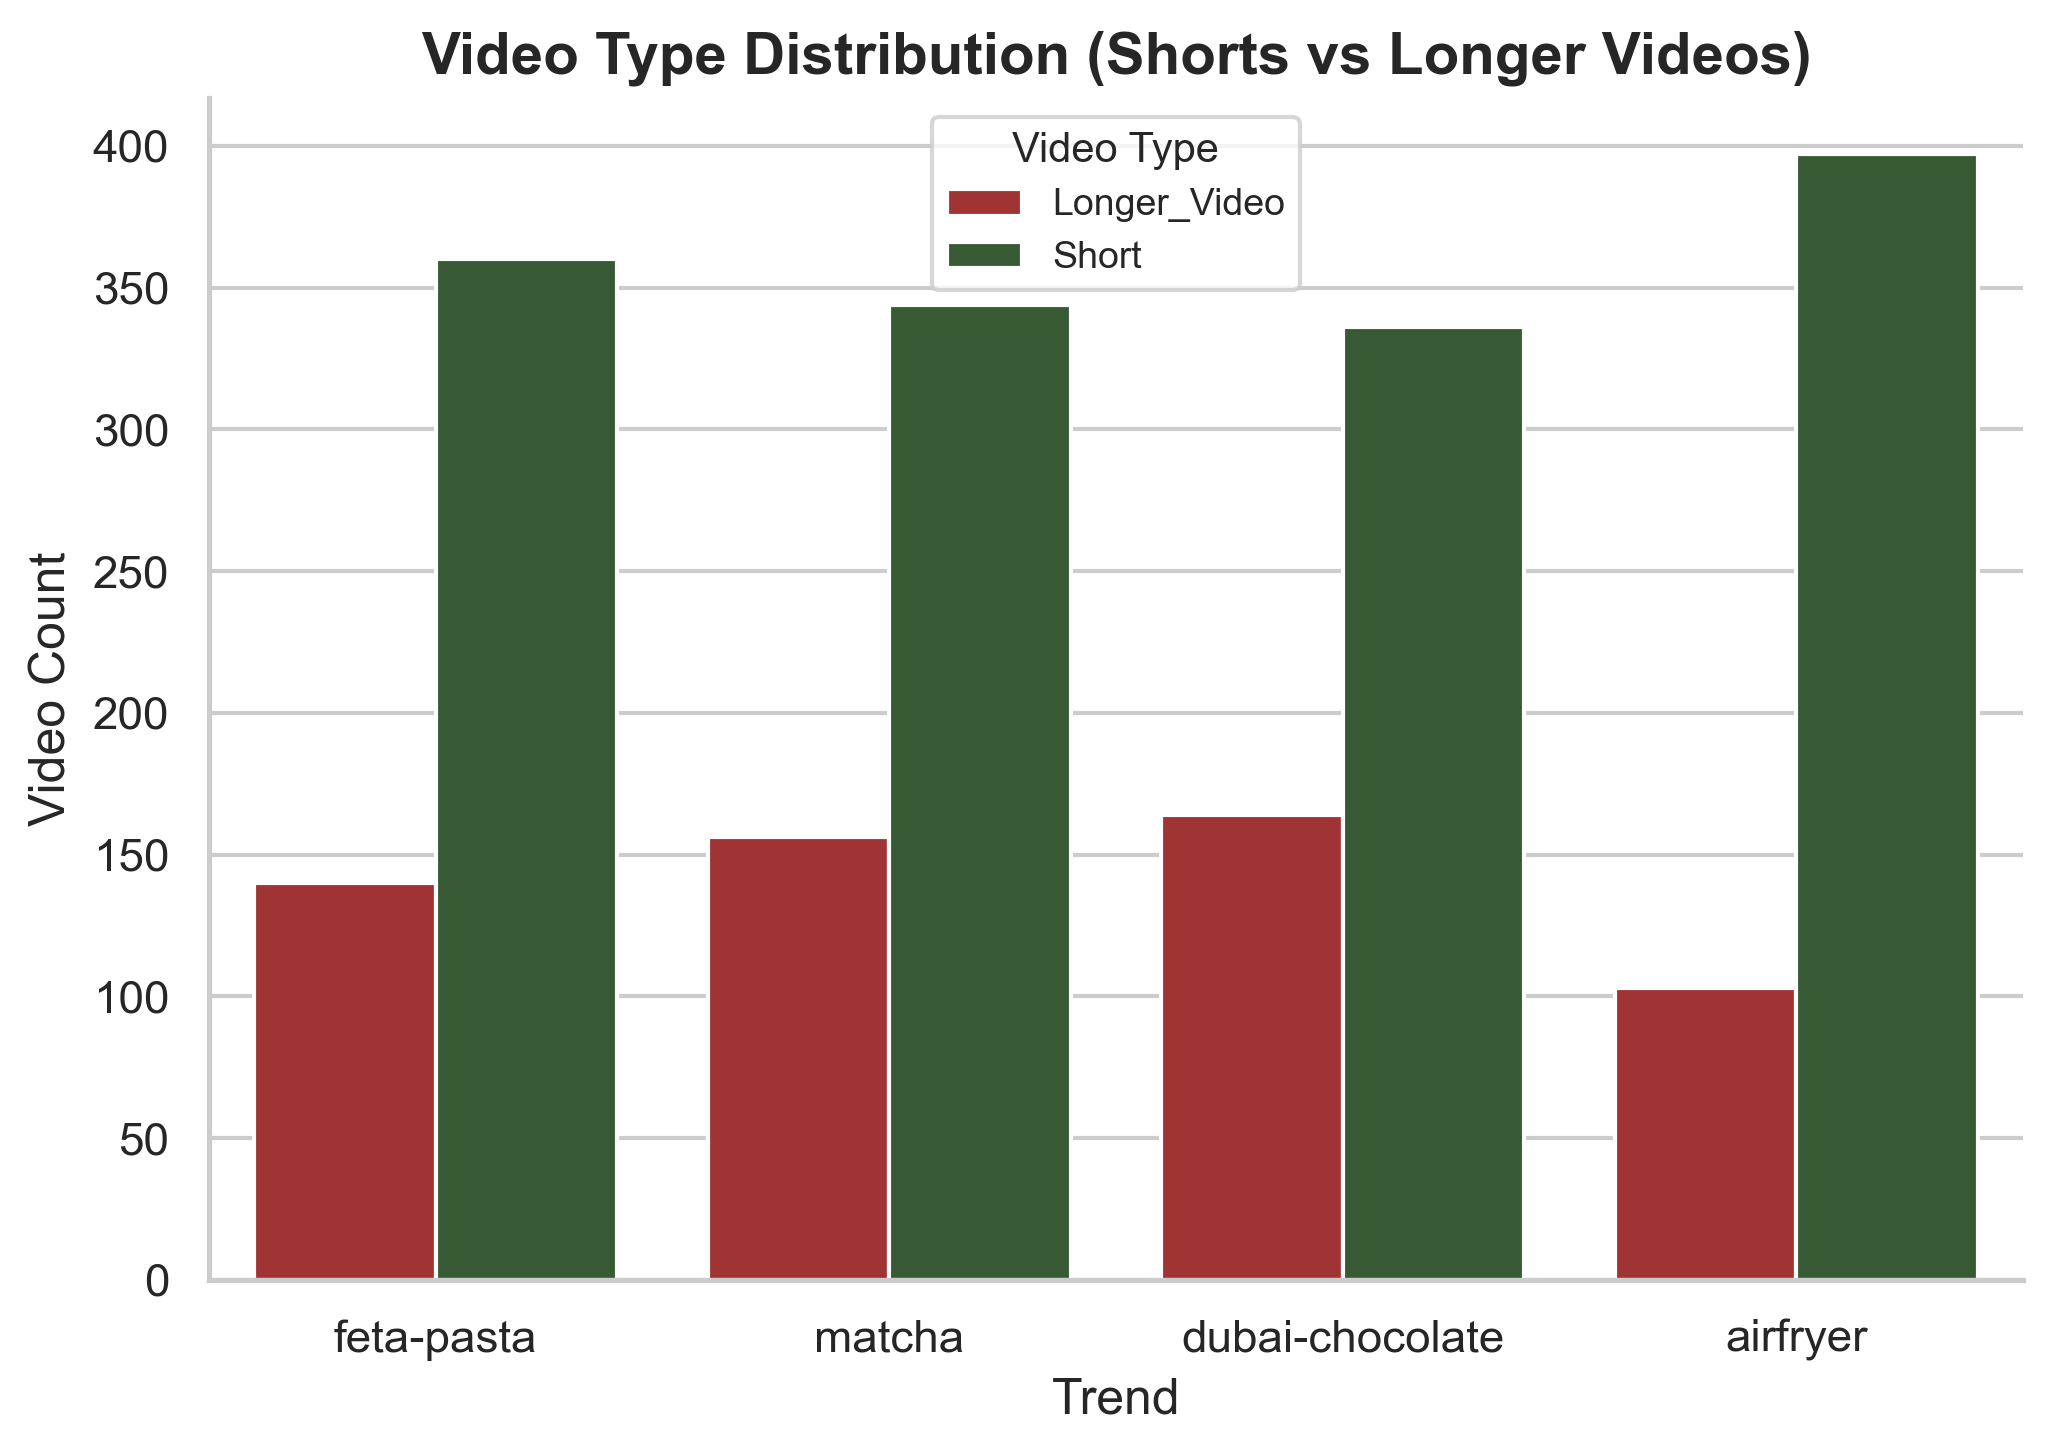
\includegraphics[width=\textwidth]{EDA_Figures/video_type.png}
        \caption{Distribution of short-form and longer videos}
        \label{fig:video_type}
    \end{minipage}
    \hfill
    % Second image
    \begin{minipage}[t]{0.48\textwidth}
        \centering
        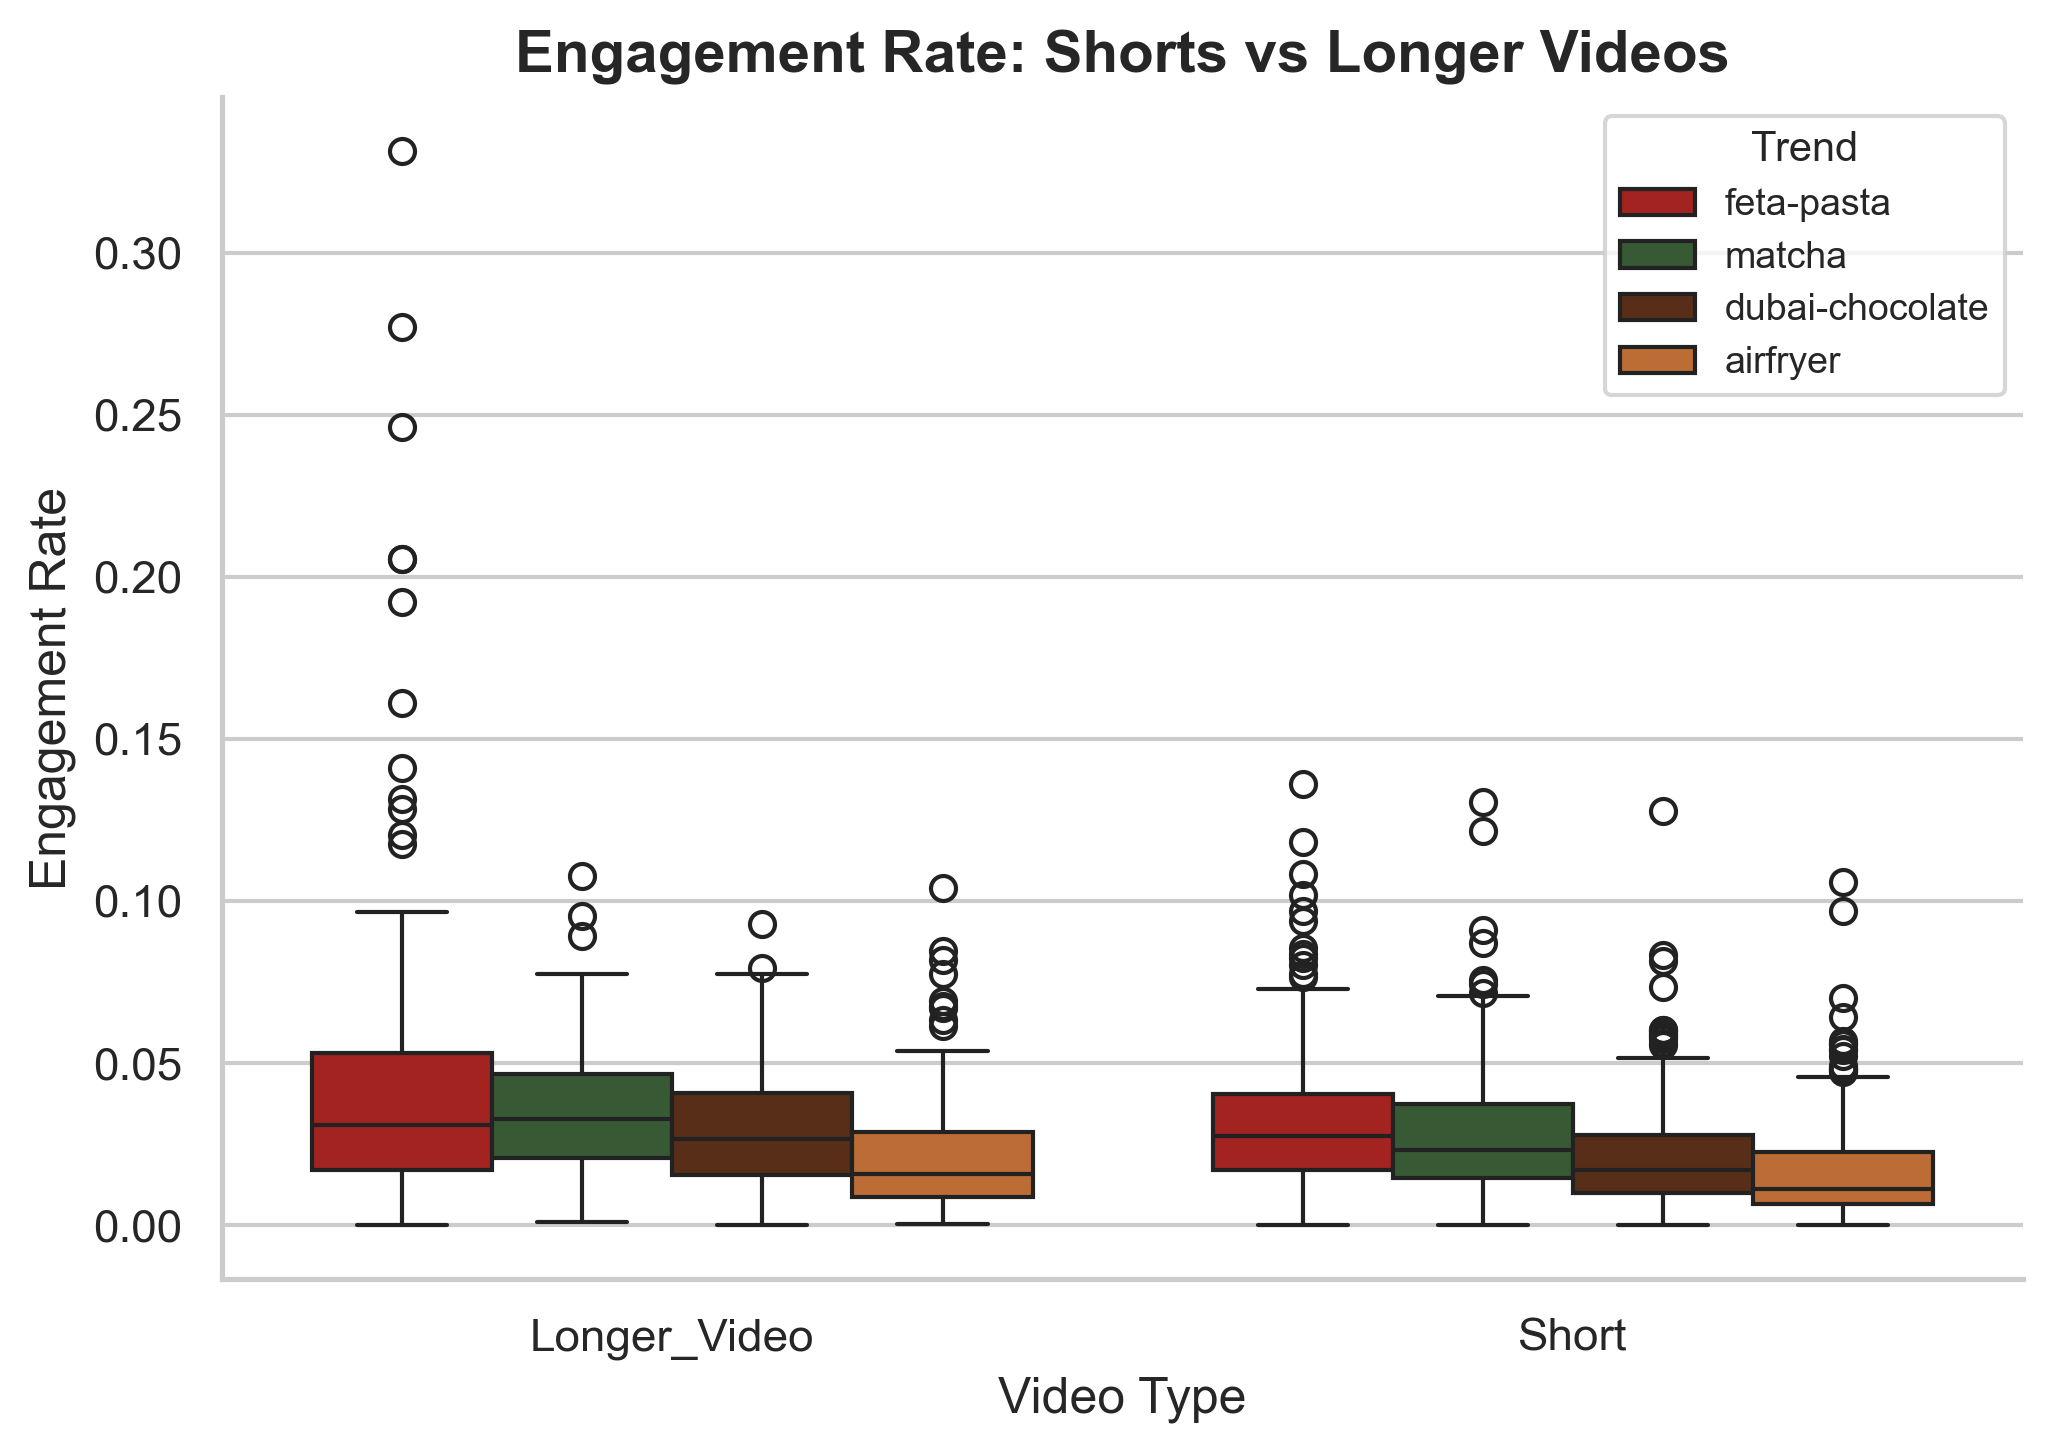
\includegraphics[width=\textwidth]{EDA_Figures/video_type2.png}
        \caption{Engagement rate between Short and longer videos}
        \label{fig:video_type2}
    \end{minipage}
\end{figure}

Across all four trends, short-form content dominates, representing roughly three-quarters of all uploads. Airfryer and Feta pasta show the largest share of Shorts, followed by Matcha and Dubai Chocolate. This pattern highlights the major role of short form content in accelerating trends. Shorts are quick to produce and consume, encouraging rapid participation in food trends. Media engagement across both types is within 0.10, showing that audience interaction remains relatively steady regardless of video length. However, longer videos show wider variation, including several high-engagement outliers above 0.10. This suggests that while shorts have consistent, moderate engagement through broad reach, longer content can achieve better interaction when it provides valuable or high-quality material. 

\begin{figure}[H]
    \centering
    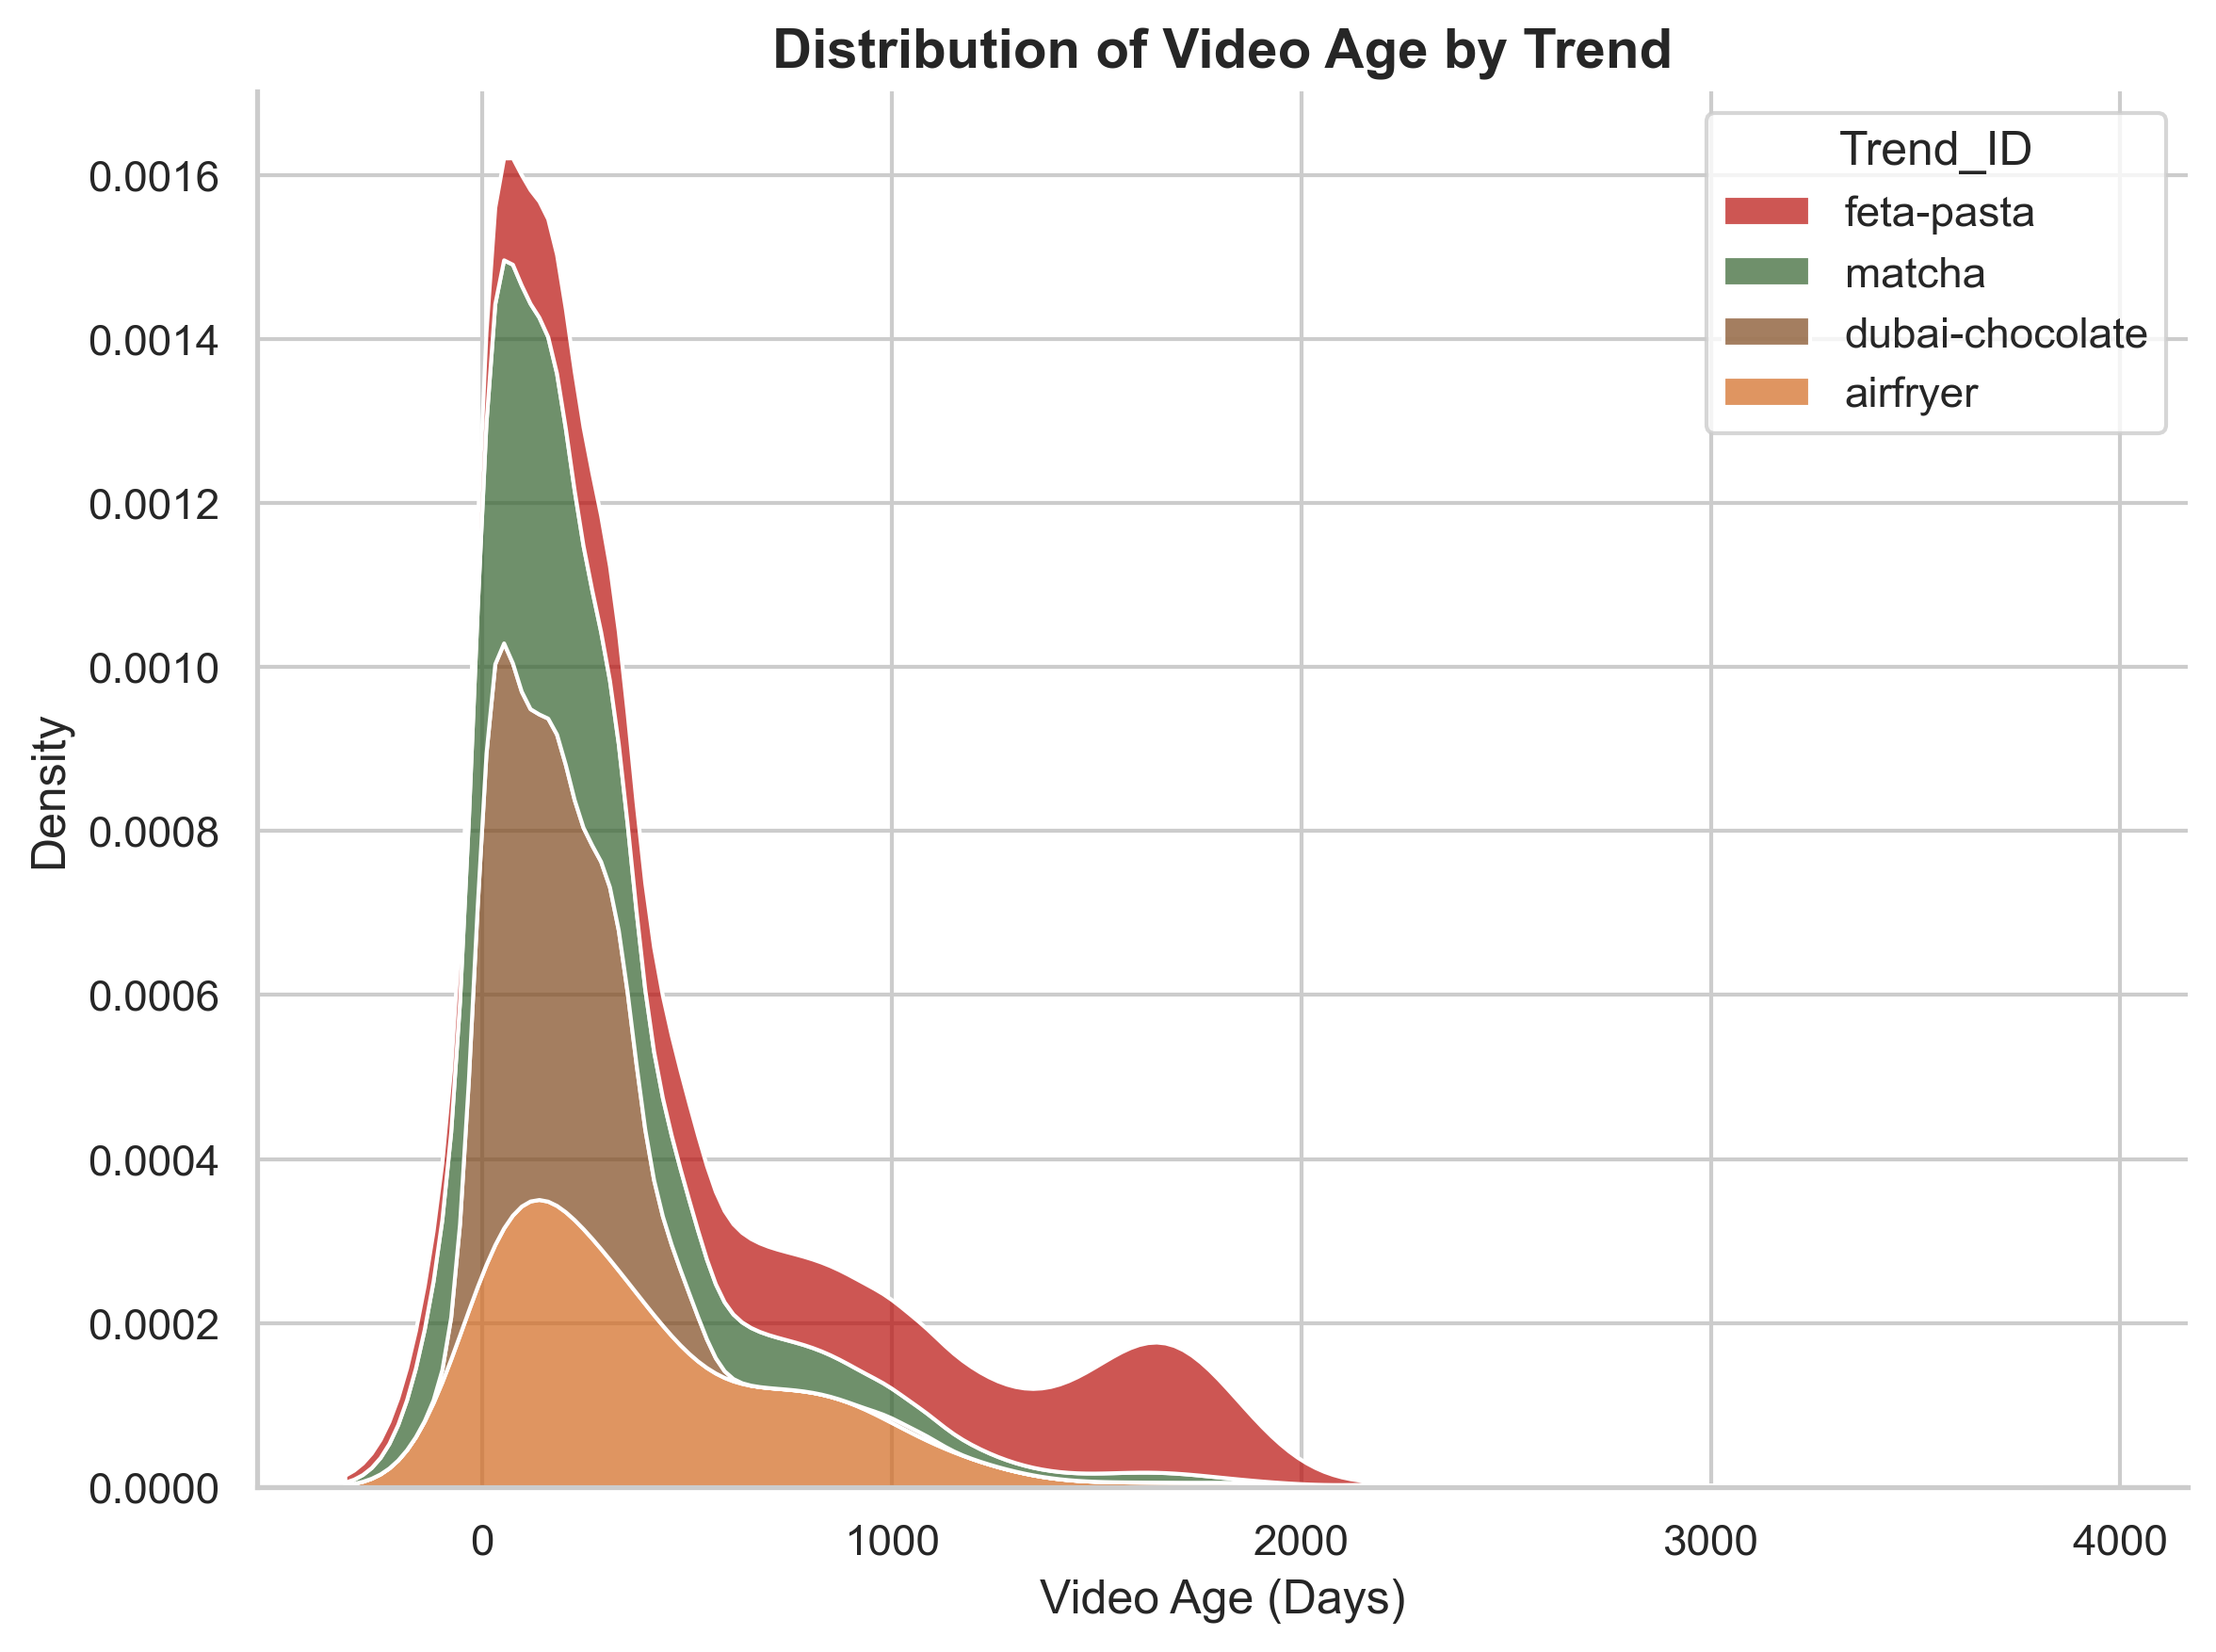
\includegraphics[width=\textwidth]{EDA_Figures/video_age.png}
    \caption{Distribution of Age of Youtube Videos}
    \label{fig:video_age}
\end{figure}

Looking at the distribution of video age for all 4 trends, most videos were uploaded within the past 2 years, with a sharp peak around 100-300 days. This suggests that food trend content is relatively recent and continues to be produced frequently. The Matcha and Dubai Chocolate trends display similar age distributions, while Feta Pasta shows an older skew due to its viral period in early 2021 and indicating limited newer uploads. In contrast, Airfryer exhibits a broader spread, reflecting its continuous popularity over time. Overall, this figure highlights the recency of most uploads, showing that content creation for these food trends remains active and current.

\begin{figure}[H]
    \centering
    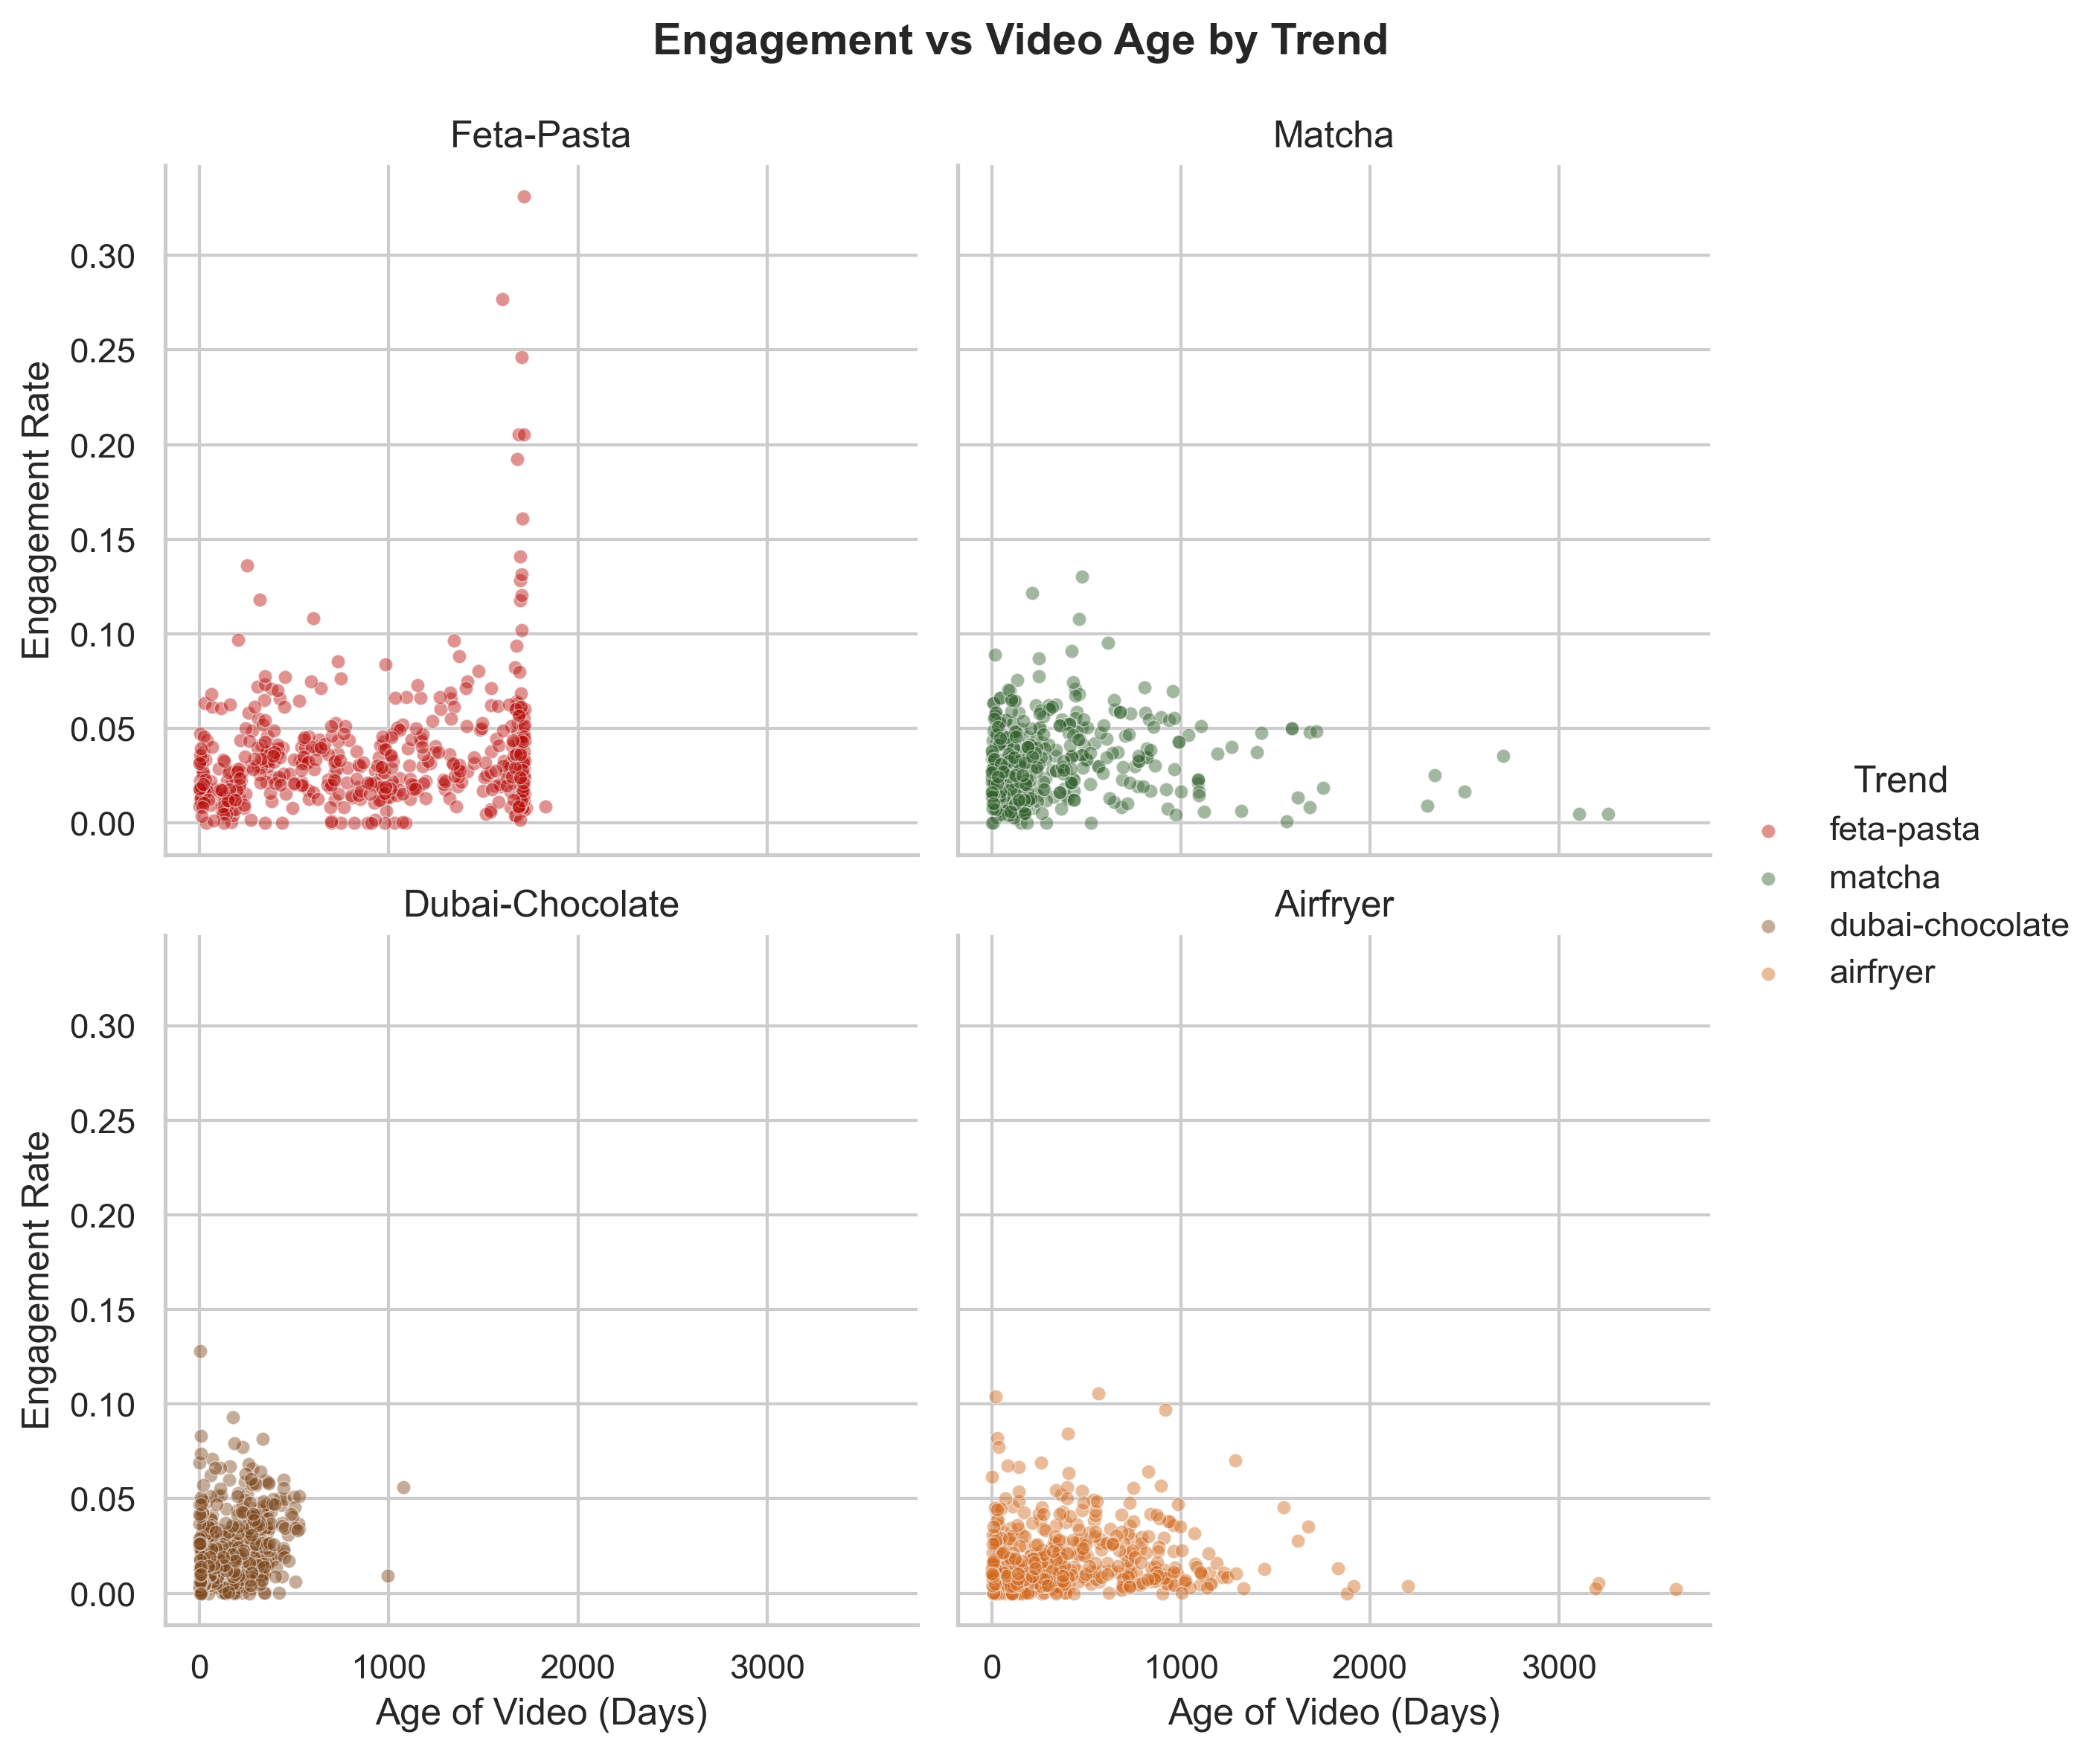
\includegraphics[width=\textwidth]{EDA_Figures/engagement_age.png}
    \caption{Comparing Engagement Rate to Age of Videos}
    \label{fig:engagement_age}
\end{figure}

After analyzing the overall distribution of video age, Figure 13 compares engagement rate to the age of videos for each trend. Across all four food trends, engagement is concentrated among newer uploads, with most of the data points contained within 1000 days. Overall the relationship between engagement and video age reinforces the time-sensitive nature of trend-driven content. While virality delivers immediate visibility, sustained engagement relies on producing content that remains culturally or practically relevant well after the initial surge of popularity. 

\begin{figure}[H]
    \centering
    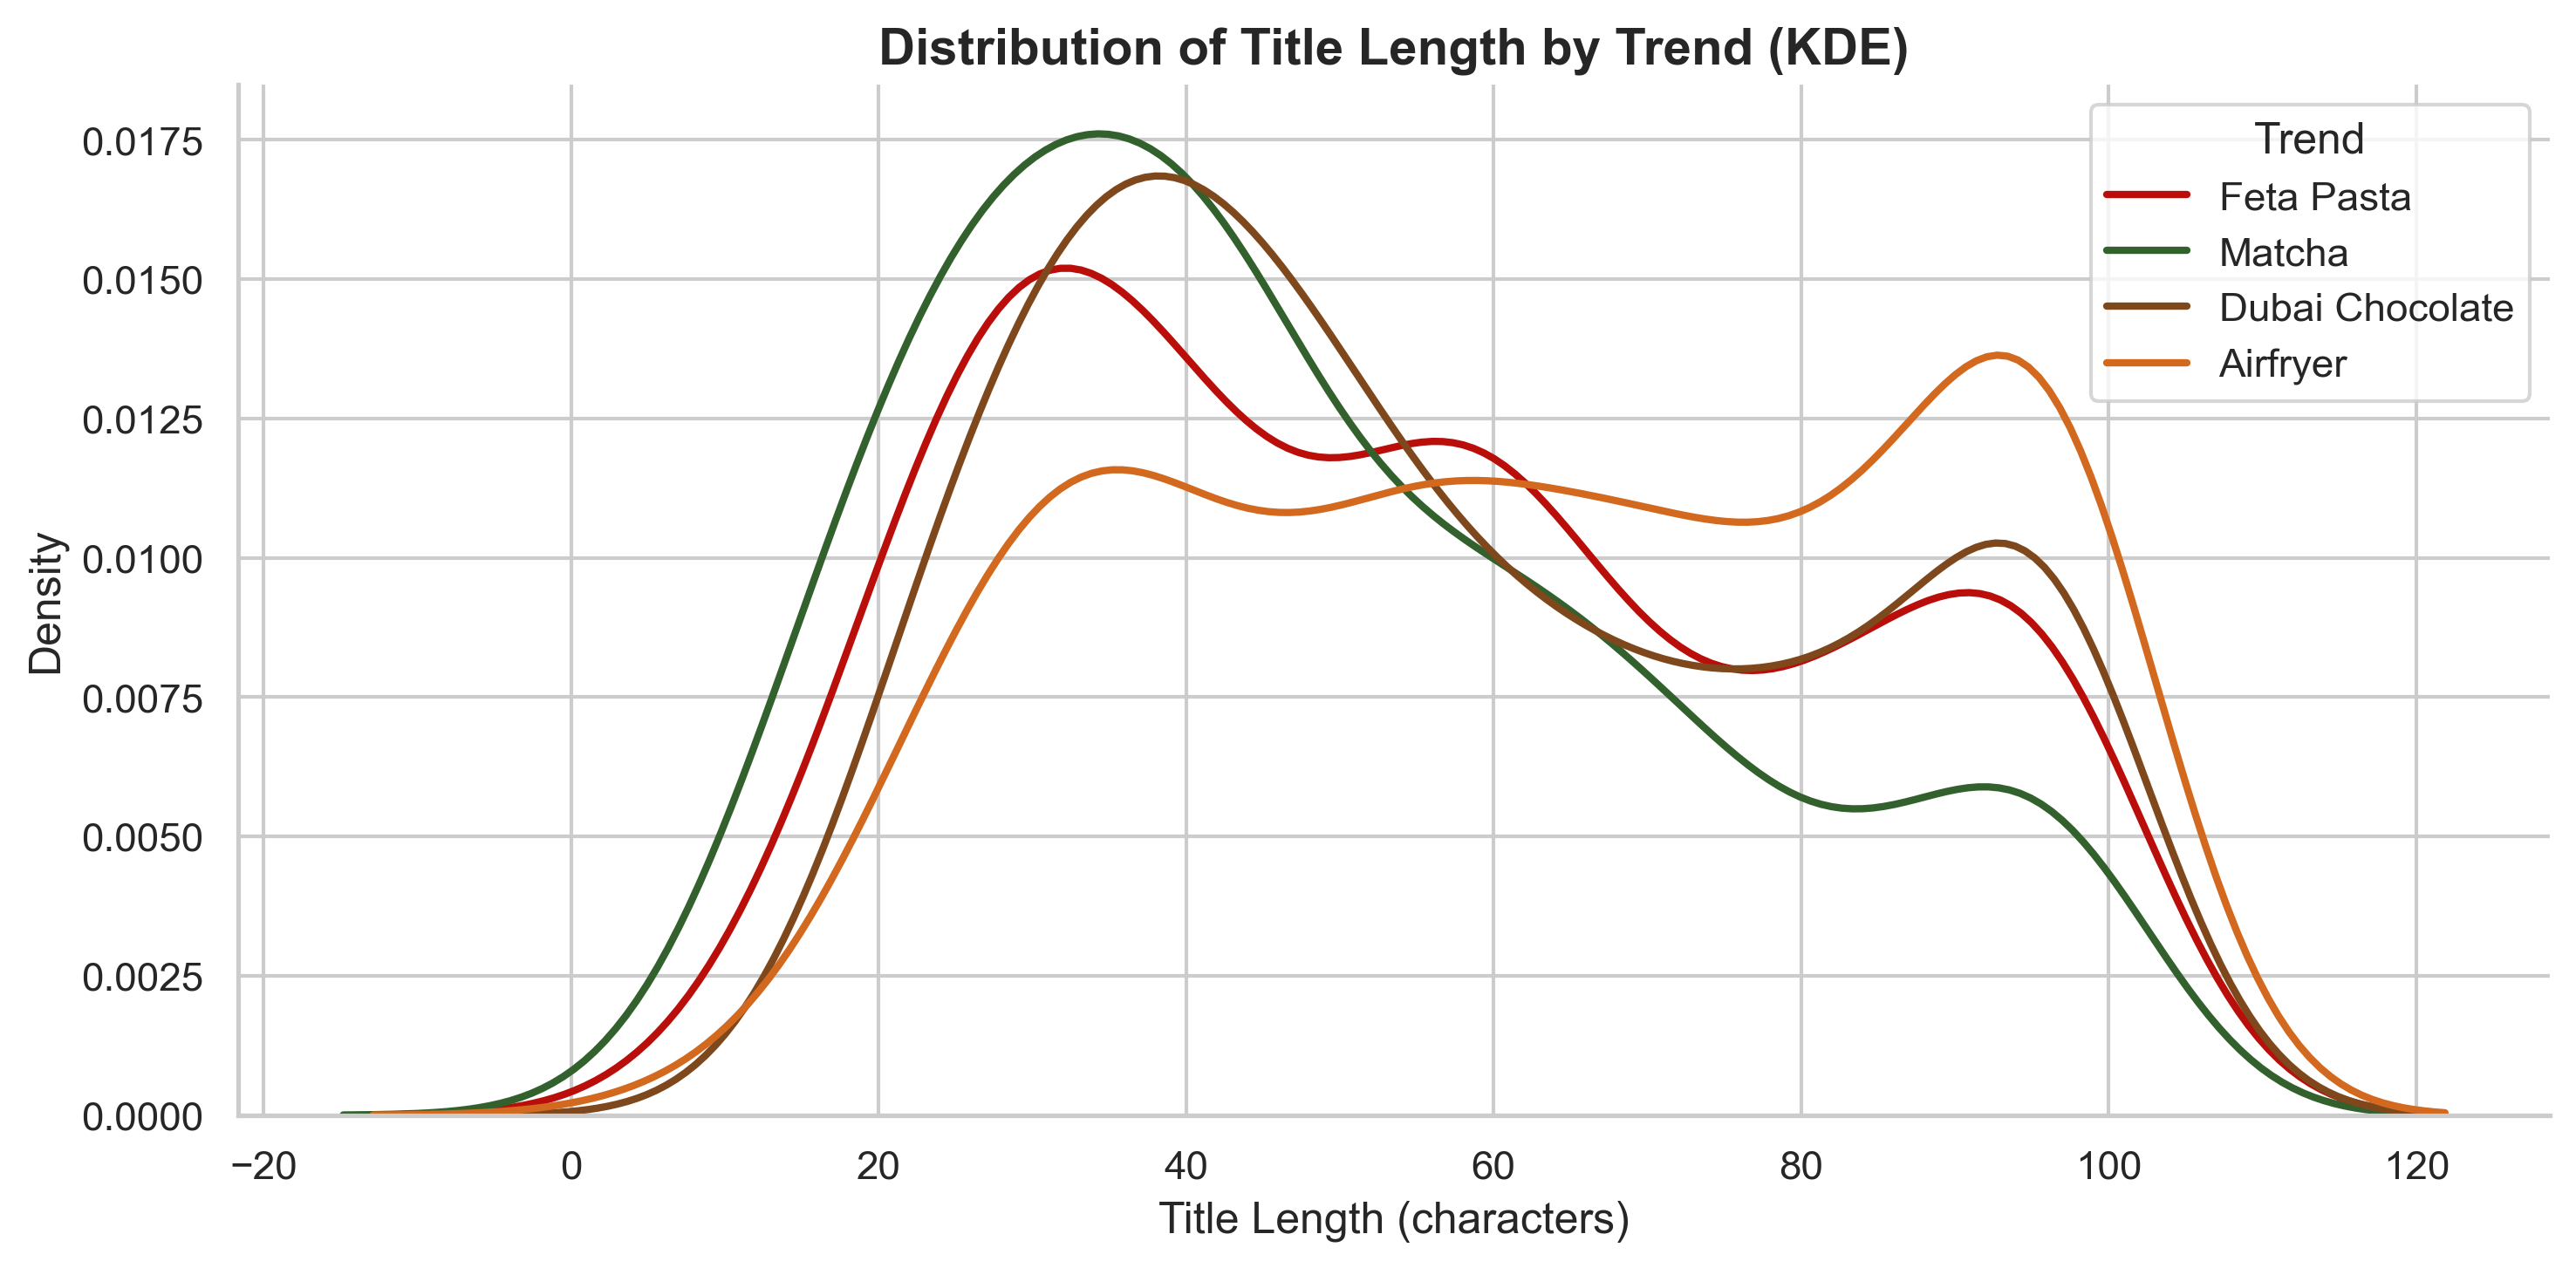
\includegraphics[width=\textwidth]{EDA_Figures/title_length.png}
    \caption{Distribution of Title Length of Youtube Videos by Trend}
    \label{fig:title_length}
\end{figure}

Figure 14 shows the distribution of title lengths across all four trends, where most video titles fall between 40 and 70 characters, suggesting that creators favor concise phrasing that balances clarity with search optimization. This range aligns with YouTube’s algorithmic preferences, which tend to prioritize shorter, keyword-rich titles in recommendations and search results.

There are, however, small differences across trends. Matcha and Dubai Chocolate videos display slightly longer average titles, possibly reflecting creators’ use of descriptive phrases to differentiate their content within saturated niches. Airfryer videos, by contrast, show a broader spread, including a secondary peak above 100 characters, suggesting that some creators rely on longer, detailed titles to emphasize recipe variations or unique preparation methods.

Overall, the title length distributions indicate that creators strategically adapt their phrasing to match audience expectations and platform behavior. While shorter titles optimize discoverability and engagement consistency, longer titles may appeal to viewers seeking depth or novelty within familiar trends.

\begin{figure}[H]
    \centering
    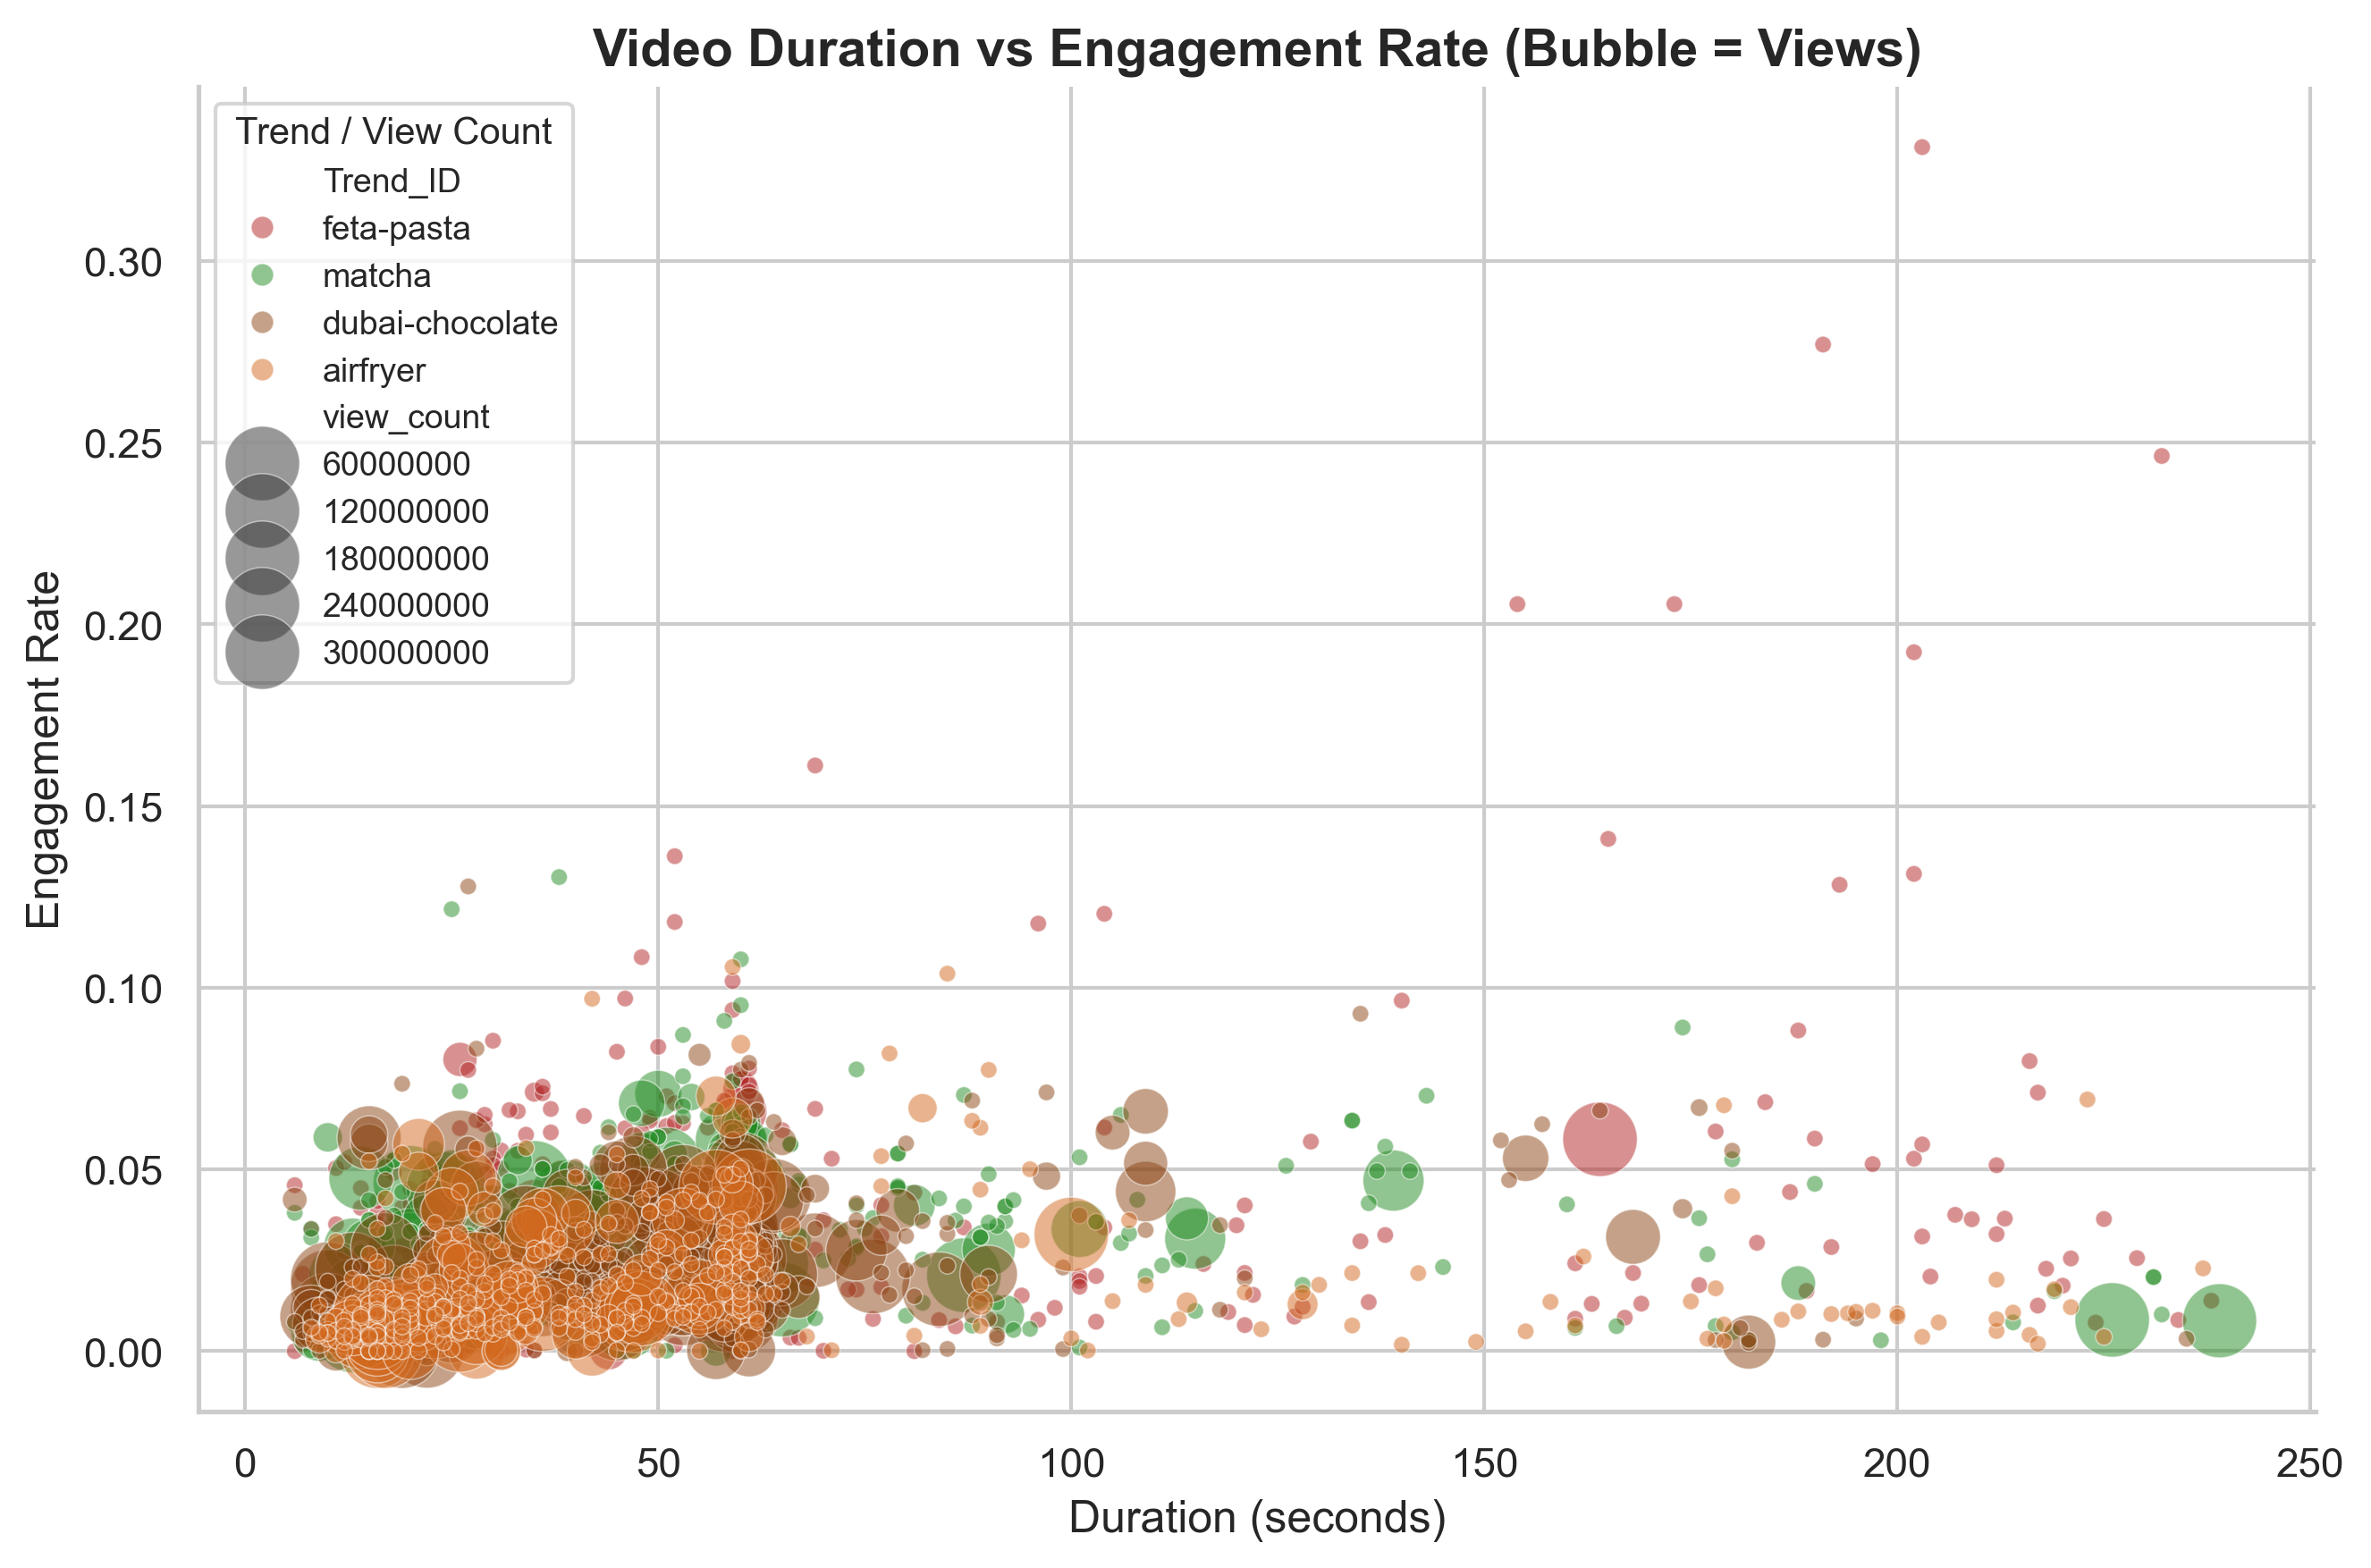
\includegraphics[width=\textwidth]{EDA_Figures/duration_engagement.png}
    \caption{Comparing Video Duration and Engagement Rates}
    \label{fig:duration_engagement}
\end{figure}

Finally, Figure 15 explores the relationship between video duration and engagement rate, with bubble size representing total view count. The plot shows that most videos cluster below 60 seconds, reflecting the dominance of short-form content across all four food trends. Engagement rates remain fairly consistent within this range, suggesting that shorter videos perform reliably well in capturing and maintaining viewer attention.

\subsection{Sentiment and Discussion Patterns}

\begin{figure}[H]
    \centering
    \includegraphics[width=\textwidth]{EDA_Figures/wordclouds.png}
    \caption{Word Clouds: Most Common Terms by Food Trends}
    \label{fig:wordclouds}
\end{figure}

After compiling Reddit discussions across food-related subreddits, Figure 15 visualizes the most frequently used terms associated with each trend. The word clouds reveal distinct thematic patterns that characterize how users discuss these foods online. Feta Pasta posts emphasize ingredients and virality, with words like “tomato,” “tiktok,” and “baked” dominating, reflecting its origin as a short-lived viral recipe. In contrast, Matcha discussions center around quality and preparation, terms such as “ceremonial,” “powder,” and “latte” highlight a focus on product grade and everyday consumption. Meanwhile, Dubai Chocolate posts frequently reference “pistachio,” “order,” and “pasabuy,” indicating a purchasing-driven conversation rather than recipe creation.


\begin{figure}[H]
    \centering
    \includegraphics[width=\textwidth]{EDA_Figures/sentiment_comparison.png}
    \caption{Sentiment Distribution Comparison}
    \label{fig:sentiment_comparison}
\end{figure}

Figure 17 illustrates how sentiment is distributed across Reddit discussions for each food trend. Across all three, the majority of posts cluster near neutrality, suggesting that most discussions are descriptive or informational rather than strongly emotional. Matcha exhibits a broader spread toward positive sentiment, aligning with its associations with health, daily lifestyle, and cultural appeal. In contrast, Feta Pasta shows slightly more neutral and negative posts, reflecting mixed reactions as enthusiasm faded following its viral peak. Dubai Chocolate maintains a narrow and moderately positive sentiment range, indicating generally favorable but limited engagement.

\begin{figure}[H]
    \centering
    \includegraphics[width=\textwidth]{EDA_Figures/average_sentiment.png}
    \caption{Average Sentiment Over Time}
    \label{fig:average_sentiment}
\end{figure}

Figure 18 tracks sentiment trajectories for each trend using daily sentiment scores and a 7-day rolling average. Matcha maintains a stable, mildly positive tone over time, demonstrating sustained community appreciation and integration into routine discussions. Feta Pasta, however, experiences sharp fluctuations, spiking during its 2021 viral moment before dropping as novelty and user interest declined. Dubai Chocolate shows a recent upward shift in 2025, reflecting growing excitement as the trend gained visibility. Together, these sentiment patterns emphasize how enduring trends sustain consistent positivity, while short-lived viral moments provoke temporary surges in enthusiasm followed by sentiment decay.


\subsection{Correlation Analysis}

\begin{figure}[H]
    \centering
    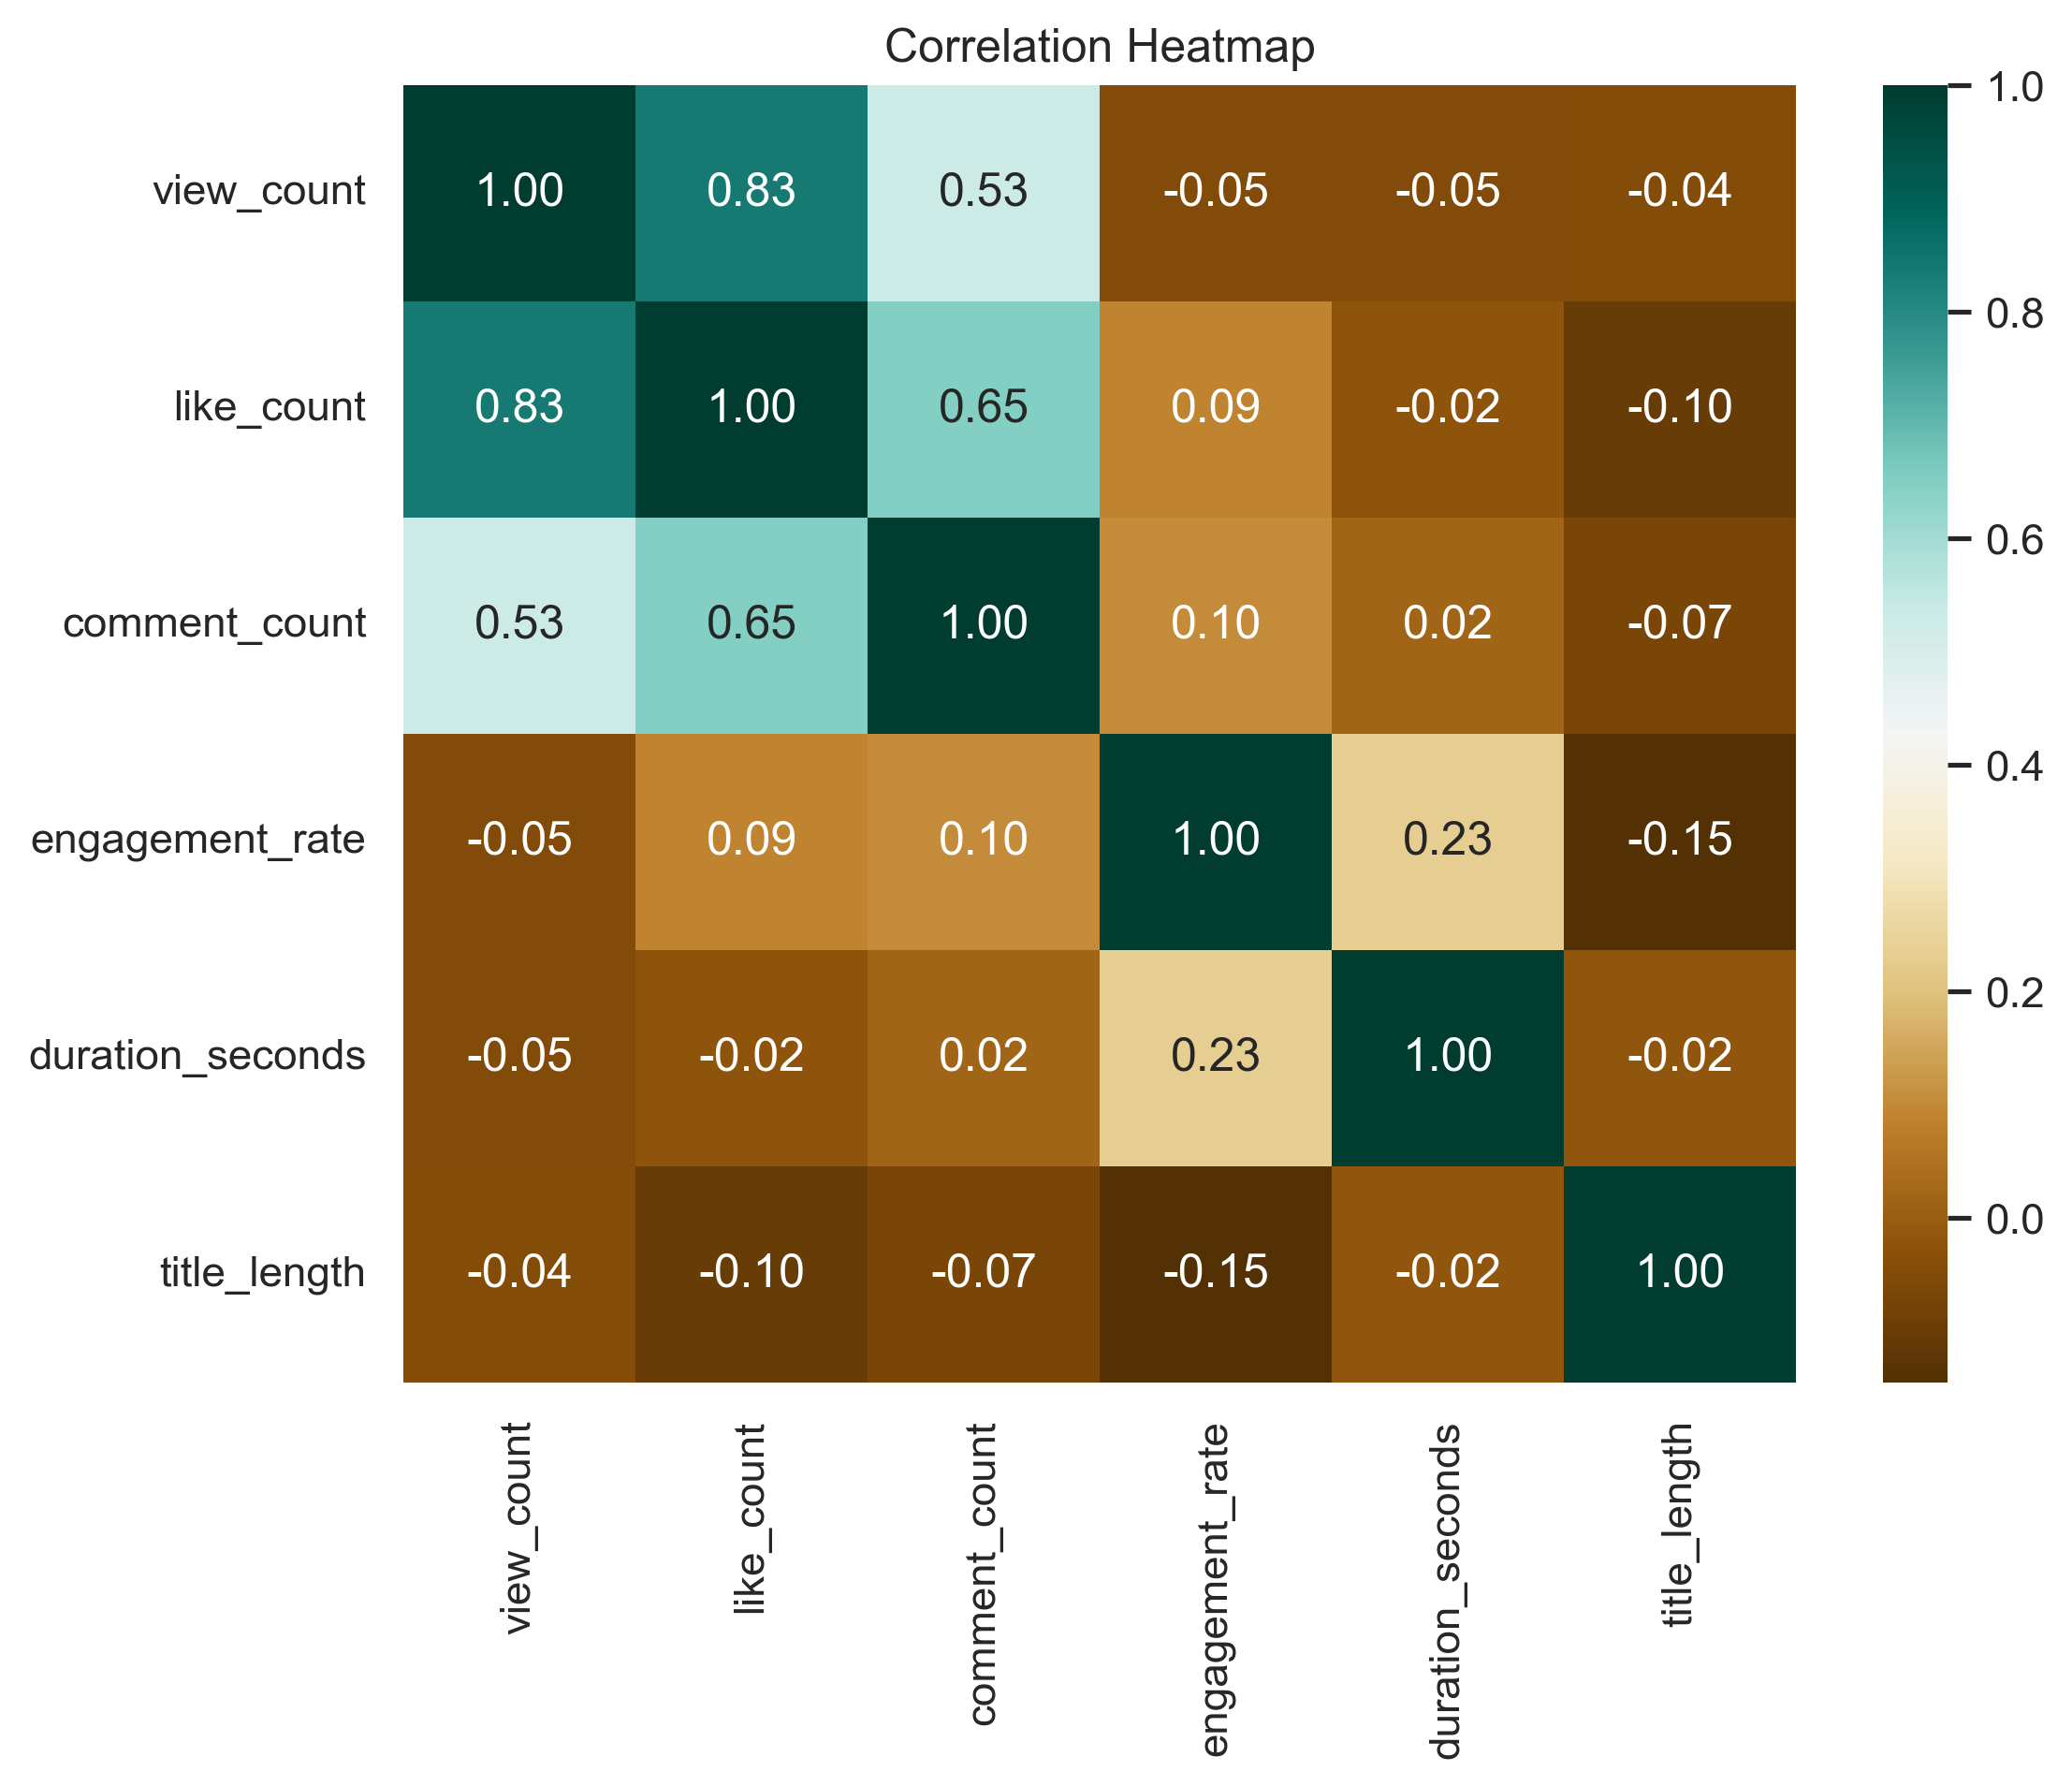
\includegraphics[width=\textwidth]{EDA_Figures/youtube_correlation.png}
    \caption{Correlation Matrix for Youtube Dataset}
    \label{fig:youtube_correlation}
\end{figure}

To examine how key numerical variables relate to one another, a correlation matrix was generated for the cleaned YouTube dataset (Figure 19). The heatmap displays pairwise correlation coefficients between engagement metrics (views, likes, comments, and engagement rate) and content attributes (duration and title length).

The results show a strong positive relationship among the three primary engagement metrics: view count, like count, and comment count. View and like counts are most highly correlated (r = 0.83), confirming that videos attracting large audiences also tend to receive more positive interactions. Comment count is moderately correlated with both views (r = 0.53) and likes (r = 0.65), suggesting that discussion intensity generally increases with visibility, though not at the same rate as passive engagement such as likes.

In contrast, engagement rate shows weak or negligible correlation with other variables, indicating that it captures a different dimension of viewer behavior—how actively audiences respond relative to total reach. This finding reinforces earlier observations that videos with high view counts do not necessarily achieve higher engagement rates.

Content-related variables, including duration and title length, exhibit little association with engagement metrics, with coefficients near zero. This suggests that neither video length nor title size directly determines audience interaction once a trend gains momentum. Instead, engagement appears to depend more on factors such as timing, content quality, and trend relevance rather than basic structural features.

Overall, the correlation analysis confirms that food trend engagement on YouTube is characterized by strong internal consistency among basic interaction metrics but independence from content format variables. This supports the interpretation that successful trend videos rely on timing and audience resonance more than on structural optimization such as video length or title composition.

\begin{figure}[H]
    \centering
    \includegraphics[width=\textwidth]{EDA_Figures/CorelationHeatmap.jpg}
    \caption{Correlation Matrix for Matcha, Dubai Chocolate and Baked Feta Cheese Pasta}
    \label{fig:engagement_age}
\end{figure}

Figure 20 illustrates the correlation matrix of worldwide Google trend interest between three food-based keywords: Matcha, Baked Feta Cheese Pasta, and Dubai Chocolate. All correlation coefficients were very low, suggesting that the variations in search interest per trend mostly displayed independence. A movement in favor or against any one trend did not dictate influence over the others in any specific time period.

The absence of significant correlation shows that each food trend yields its own distinct lifecycle of discovery and virality, driven by its own cultural or social media determinants. Baked Feta Cheese Pasta, for example, became popular based on infrequent bursts of virality, in contrast to Matcha and Dubai Chocolate that appear more sporadic or region-based in their trends. Collectively, the correlation analysis confirms each food trend emerged and developed independently of one another in the worldwide online trend landscape.

\newpage

\section{Implications and Next Steps}
This exploratory analysis conducted across Youtube \citep{youtube_api}, Reddit \citep{reddit_api_praw}, and Google Trends \citep{pytrends_api} reveal how digital food trends follow distinct lifecycles of emergence, peak, and decline. Youtube acts as a medium for visual engagement, Reddit reflects conversational and sentiment-based depth, and Google Trends captures population-level searches over time. Combining these perspectives provides a holistic view of how trends move from online novelty to global phenomena. 

While the current analysis offers meaningful insights, the process of data collection and pre-processing proved to be both time-consuming and technically complex. Unlike readily available static datasets, our approach relied on live data acquisition through public APIs: YouTube Data API v3 \citep{youtube_api}, Reddit API (PRAW) \citep{reddit_api_praw}, and Google PyTrends \citep{pytrends_api}, which required multiple iterations of data cleaning, rate-limit handling, and authentication. These constraints extended project timelines but also ensured that the analysis was based on real-time, authentic digital activity rather than archived or outdated samples.

Due to time constraints and API limitations, we were unable to develop regional visualizations using Google PyTrends, such as country-level heatmaps or diffusion maps to illustrate the geographical spread of food trends. Future work will address this gap by expanding the dataset with additional regional queries to explore cross-cultural differences in trend adoption and intensity.

Another next step involves performing cross-dataset analyses to measure the relationships between public search interest (Google Trends), video engagement patterns (YouTube), and conversational sentiment (Reddit). By aligning these datasets temporally, we can test whether spikes in content creation precede increases in search interest or follow social media virality.

Finally, the long-term objective is to develop a predictive model capable of estimating a trend’s peak popularity and longevity based on early engagement indicators. This model would combine sentiment, search volume, and video activity data to predict whether a trend will become viral, sustain steady growth, or decline rapidly.

\newpage
\bibliographystyle{plain}
\bibliography{references}   

\end{document}
